\documentclass{patmorin}
 
\usepackage{pat}
\usepackage[utf8]{inputenc}
\usepackage[noend]{algorithmic}
\usepackage{subcaption}
\usepackage{enumitem}
\usepackage{url}
\usepackage{comment}

\newcommand\numberthis{\addtocounter{equation}{1}\tag{\theequation}}

% taken from http://goo.gl/JVNEL2
\newtheorem{innercustomthm}{Theorem}
\newenvironment{customthm}[1]
  {\renewcommand\theinnercustomthm{#1}\innercustomthm}
  {\endinnercustomthm}

\title{\MakeUppercase{Encoding Arguments}\thanks{This research is partially funded by NSERC.}}
\author{Pat Morin, Wolfgang Mulzer, and Tommy Reddad}
\date{}

\begin{document}
\begin{titlepage}
\maketitle


\begin{abstract}
  \setlength{\baselineskip}{15.84pt}

  This expository article surveys ``encoding arguments.'' In their
  most most basic form an encoding argument proves an upper bound on
  the probability of an event using the fact a uniformly random choice
  from a set of size $n$ can not be encoded with fewer than $\log_2 n$
  bits on average.

  We survey many applications of this basic argument, give a
  generalization of this argument for the case of non-uniform
  distributions, and give a rigorous justification for the use of
  non-integer codeword lengths in encoding arguments.  These latter
  two results allow encoding arguments to be applied more widely and
  to produce tighter results.
\end{abstract}

\keywords{Encoding arguments, entropy, Kolmogorov complexity, 
          incompressibility, random graphs, expanders, \ldots}

\end{titlepage}
\pagenumbering{roman}
\tableofcontents
\newpage
\pagenumbering{arabic}

\section{Introduction}
\setlength{\baselineskip}{15.84pt}

There is no doubt that probability theory plays a fundamental role in
computer science: Some of the fastest and simplest fundamental
algorithms and data structures are randomized; average-case analysis
of algorithms relies entirely on tools from probability theory; and
many difficult combinatorial questions have strikingly simple
solutions using probabilistic arguments.

Unfortunately, many of these beautiful results are inaccessible to
most computer scientists because of a view that ``the math is too
hard.''  For instance, the 2013 edition of ACM/IEEE Curriculum
Guidelines for Undergraduate Degree Progams in Computer Science does
not require a full course in probability theory
\cite[Page~50]{computing-curricula:computer}. Indeed, the report
recommends a total of 6 Tier-1 hours and 2 Tier-2 hours spent on
discrete probability, as part of the discrete structures curriculum
\cite[Page~77]{computing-curricula:computer}.

In this expository paper, we survey applications of ``encoding
arguments'' that tranforms the problem of upper-bounding the
probability of a specific event, $\mathcal{E}$, into the problem of
devising a code for the set of elementary events in $\mathcal{E}$.
Encoding arguments have several advantages over traditional
probabilistic analysis:

\begin{enumerate}
\item Encoding arguments are almost ``probability-free.''  Except for
  applying a simple \emph{Uniform Encoding Lemma}, there is no
  probability involved.  In particular, there is no chance to make
  common mistakes such as multiplying probabilities of non-independent
  events or (equivalently) multiplying expectations.

  The proof of the Uniform Encoding Lemma itself is trivial and the
  only probability it uses is that the fact, if a finite set $X$
  contains $r$ special elements and we pick an element uniformly at
  random from $X$, then the probability of picking a special element
  is $r/|X|$.

\item Encoding arguments usually yield strong results;
  $\Pr\{\mathcal{E}\}$ typically decreases at least exponentially in
  the parameter of interest. Traditionally, these strong concentration
  results require (at least) careful calculations on probabilities of
  independent events and/or the application of concentration
  inequalities.  The subject of concentration inequalities is advanced
  enough to be the topic of entire textbooks
  \cite{boucheron.lugosi.ea:concentration,dubhashi.panconesi:concentration}.
  
\item Encoding arguments are natural for computer scientists. They
  turn a probabilistic analysis problem into the problem of designing
  an efficient code---an algorithmic problem. Consider the following
  two problems:
  \begin{enumerate}

  \item Prove an upper-bound of $1/n^{\log n}$ on the probability that
    a random graph on $n$ vertices contains a clique of size $k=\lceil
    4\log n\rceil$.\footnote{Since we are overwhelmingly concerned with
    binary encoding, we will
    agree now that the base of logarithms in $\log x$ is $2$, except when
    explicitly stated otherwise.}

  \item Design a encoding for graphs on $n$ vertices so that a graph,
    $G$, that contains a clique of size $k=\lceil 4\log n\rceil$ is
    encoded using at most $\binom{n}{2}-\log^2 n$ bits. (Note: Your
    encoding and decoding algorithms don't have to be efficient, just
    correct.)
  \end{enumerate}
  Many computer science undergraduates would not know where to start
  on the first problem.  Even a good student who realizes that they
  can use Boole's Inequality will still be stuck wrestling with the
  formula $\binom{n}{4\log n}2^{-\binom{4\log n}{2}}$.
\end{enumerate}

Our motivation for this work is that encoding arguments are an easily
accessible, yet versatile tool for answering many questions.  Most of
these arguments can be applied after learning almost no probability
theory beyond the Encoding Lemma mentioned above.

The remainder of this article is organized as follows: In
\secref{uel}, we present necessary background, including the
\emph{Uniform Encoding Lemma}, which is the basis of most of our
encoding arguments.  \Secref{applications-i} presents applications of
the Uniform Encoding Lemma to a variety of problems.  \Secref{nuel}
presents a more general Non-Uniform Encoding Lemma that can handle a
larger variety of applications, some of which are presented in
\secref{applications-ii}.  \Secref{el} presents an alternative view of
encoding arguments, justifying the use of non-integer codeword
lengths.  \Secref{summary} summarizes and concludes with some
directions for future research.

\section{Background}
\seclabel{uel}

This section presents the necessary background on prefix-free codes
and binomial coefficients.

\subsection{Prefix-free Codes and the Uniform Encoding Lemma}

A finite length \emph{string} over an alphabet $\Sigma$ is either the
empty string or an element of $\Sigma^k$ for some $k \in \N$. The
expression $\{0, 1\}^*$ denotes the set of all finite length binary
(or bit) strings. For a string, $s$, we use $|s|$ to denote the length of
$s$.  A bit string of length $n$ will be called an $n$-bit
string. A \emph{code} $C\from X\to \{0,1\}^*$ is a one-to-one function
from a set $X$ to the set of finite length binary strings.  The
elements of the range of $C$ are called $C$'s \emph{codewords}.  In
most cases, there are some elements of the set $X$ that are not of
interest to us.  In these cases, we consider partial codes. A
\emph{partial code} $C\from X\nrightarrow \{0,1\}^*$ is a one-to-one
partial function.  When discussing partial codes we will use the
convention that $|C(x)|=\infty$ if $x$ is not in the domain of $C$.

A (partial) code $C$ is \emph{prefix-free} if, for every pair
$x\neq y$ in the domain of $C$, the binary string $C(x)$ is not a
prefix of $C(y)$.  It can be helpful to think of prefix-free codes as
(rooted ordered) binary trees whose leaves are labelled with the
elements of $X$.  The codeword for a particular $x\in X$ is obtained
by tracing the root-to-leaf path leading to $x$ and outputting a 0
(respectively, 1) each time this path goes from a parent to its left
(respectively, right) child. (See \figref{bintree}.)

\begin{figure}
  \centering{\includegraphics{bintree}}
  \caption{A prefix-free code for the set
    $X=\{\mathtt{a},\mathtt{b},\mathtt{c},\mathtt{d},\mathtt{e},\mathtt{f}\}$
    and the corresponding leaf-labelled binary tree (which can also be
    viewed as a partial prefix-free code for the set
    $\{\mathtt{a},\mathtt{b},\mathtt{c},\ldots,\mathtt{z}\}$).}
  \figlabel{bintree}
\end{figure}

If $C$ is prefix-free, then the number of $C$'s codewords that have
length at most $k$ is not more than $2^k$. To see this why this is so,
observe that $C$ can be modified into a code $\hat C$, in which every
codeword of length $\ell <k$ is extended---by appending $k-\ell$
zeros---so that it has length exactly $k$. The prefix-freeness of $C$
ensures that $\hat C$ is also a prefix-free code. The number of $\hat
C$'s codewords of length $k$ is equal to the the number of $C$'s
codewords of length at most $k$; since codewords are just binary
strings, there are not more than $2^k$ of these.

Observe that every finite set $X$ has a prefix-free code in which
every codeword has length $\lceil\log |X|\rceil$. We simply enumerate
the elements of $X$ in some order $x_0,x_1,\ldots,x_{|X|-1}$ and
assign to each $x_i$ the binary representation of $i$ (padded with
leading zeros), which has length $\lceil\log |X|\rceil$, since
$i\in\{0,\ldots,|X|-1\}$.  We will use this type of \emph{fixed-length
  code} implicitly in many arguments.


As we will see, the following lemma, which is folklore, is
surprisingly versatile:
\begin{lem}[Uniform Encoding Lemma]\lemlabel{uel}
  Let $C\from X\nrightarrow \{0,1\}^*$ be a partial prefix-free
  code. If an element $x\in X$ is chosen uniformly at random, then
  \[
    \Pr\{|C(x)|\le \log|X|-s\}\le 2^{-s} \enspace .
  \]
\end{lem}

\begin{proof}
  Let $k=\log|X|-s$ and recall that $C$ has at most $2^{k}$ codewords
  of length at most $k$.  Since $C$ is one-to-one each such codeword
  has at most one preimage in $X$.  Since $x$ is chosen uniformly at
  random from $X$, the probability that it is the preimage of one of
  these short codewords is at most
  \[
  \frac{2^k}{|X|} = \frac{2^{\log|X|-s}}{|X|} = 2^{-s} \enspace
  . \qedhere
  \]
\end{proof}

\subsection{Runs in Binary Strings}

As a warm-up exercise to illustrate the use of the Uniform Encoding
Lemma we will show that a random $n$-bit string is unlikely to contain
a run of significantly more than $\log n$ one bits.  (See
\figref{runs-i}.)

\begin{figure}
  \centering{\includegraphics{runs-i}}
  \caption{Illustration of \thmref{runs-i} and its proof.}
  \figlabel{runs-i}
\end{figure}

\begin{thm}\thmlabel{runs-i}
  Let $x=(x_1,\ldots,x_n)\in\{0,1\}^n$ be chosen uniformly at random
  and let $t = \ceil{\ceil{\log n} + s}$. Then, the probability that
  there exists an $i\in\{1,\ldots,n-t+1\}$ such that
  $x_i=x_{i+1}=\cdots=x_{i+t-1}=1$ is at most $2^{-s}$.
\end{thm}

\begin{proof}
  We will prove this theorem by constructing a partial prefix-free
  code for strings having a run of $t$ or more ones.  For such a
  string $x=(x_1,\ldots,x_n)$ let $i$ be the minimum index such that
  $x_i=x_{i+1}=\cdots=x_{i+t-1}=1$. The codeword $C(x)$ for $x$ is the
  binary string that consists of the ($\lceil\log n\rceil$-bit binary
  encoding of the) index $i$ followed by the $n-t$ bits
  $x_1,\ldots,x_{i-1},x_{i+t},\ldots,x_n$. (See \figref{runs-i}.)

  Observe that $C(x)$ has length 
  \[
    \lceil\log n \rceil + n - t \le n-s \enspace .
  \]
  It is easy to check that, for any such $x$, we can reconstruct
  $(x_1,\ldots,x_n)$ from $C(x)$, so $C$ is a partial code whose
  domain is the set of binary strings of length $n$ having a run of
  $t$ or more ones.  It is also easy to see that $C$ is prefix free,
  since all codewords are unique and have the same length.

  Now, $x$ was chosen uniformly at random from a set of size $2^{n}$.
  Therefore, by the Uniform Encoding Lemma, the probability that there
  exists any index $i\in\{1,\ldots,n-t-1\}$ such that
  $x_i=x_{i+1}=\cdots=x_{i+t-1}=1$ is at most
  \[
    \Pr\{|C(x)|\le n-s\} \le 2^{-s} \enspace . \qedhere 
  \]
\end{proof}

Simple as it is, the proof of \thmref{runs-i} contains the main ideas
used in most encoding arguments:

\begin{enumerate}
\item The arguments usually show that a particular \emph{bad event} is
  unlikely. In \thmref{runs-i} the bad event is the occurrence of a
  substring of $t$ consecutive ones.

\item The code is partial prefix-free code whose domain contains the
  set of bad events. In this case, the code $C$ is only capable of
  encoding strings containing a run of $t$ consecutive ones.

\item The code usually begins with a concise description of the bad
  event, and is then followed by a straightforward encoding of the
  information that is not implied by the bad event. In
  \thmref{runs-i}, the bad event is completely described by the index
  $i$ at which the run of $t$ one bits begins, and this implies that
  the bits $x_i,\ldots,x_{i+t-1}$ are all equal to 1, so these bits do
  not need to be specified in the second part of the codeword.
\end{enumerate}

\subsection{A Note on Ceilings}

Note that \thmref{runs-i} also has an easy proof using the union
bound: If we let $\mathcal{E}_i$ denote the event
$x_i=x_{i+1}=\cdots=x_{i+t}=1$, then
\begin{align*}
  \Pr \bigcup_{i=0}^{n-t-1} \mathcal{E}_i
  & \le \sum_{i=0}^{n-t-1} \Pr\mathcal{E}_i  \tag{using the union bound}\\
  & = \sum_{i=0}^{n-t-1} 2^{-t}  \tag{using the independence of the $x_i$'s}\\
  & \le n2^{-t}  \tag{the sum has $n-t\le n$ identical terms}\\
  & = n2^{-\lceil\log n\rceil-s}  \tag{from the definition of $t$}\\
  & \le 2^{-s} \enspace .
\end{align*}
This traditional proof also works with the sometimes smaller value
$t=\ceil{\log n+s}$ (note the lack of a ceiling over the logarithmic
term), in which case the final inequality becomes an equality.

In the encoding proof of \thmref{runs-i}, the ceiling in the
expression for $t$ is an artifact of encoding the integer $i$ which is
taken from a set of size $n$. When sketching an encoding argument, we
think of this as requiring $\log n$ bits but when it comes time to
carefully write down a proof we include a ceiling over this term since
bits are a discrete quantity.

In \secref{el}, however, we will see that the informal intuition we
use in blackboard proofs is actually valid; we can think of encoding
$i$ using $\log n$ bits even if $\log n$ is not an integer.  In
general we can imagine encoding a choice from among $r$ options using
$\log r$ bits for any $r\in\N$.  From this point onwards, we omit
ceilings this way in all our theorems and proofs. This makes
calculations simpler and provides tighter results.  For now, it allows
us to state the following cleaner version of \thmref{runs-i}:

\begin{customthm}{\ref*{thm:runs-i}b}\thmlabel{runs-ii}
  Let $x=(x_1,\ldots,x_n)\in\{0,1\}^n$ be chosen uniformly at random
  and let $t = \ceil{\log n + s}$. Then, the probability that there
  exists an $i\in\{1,\ldots,n-t+1\}$ such that
  $x_i=x_{i+1}=\cdots=x_{i+t-1}=1$ is at most $2^{-s}$.
\end{customthm}

\subsection{Encoding Sparse Bit Strings}\seclabel{sparse-bit-strings}

At this point we should also point out an extremely useful trick that
we can use for encoding sparse bit strings. For any $\alpha\in(0,1)$,
there exists a code $C_\alpha\from \{0,1\}^n\rightarrow \{0,1\}^*$
such that, for any bit string $x\in\{0,1\}^n$ having $n_1(x)$ ones and
$n_0(x)$ zeros,
\begin{equation}
  |C_\alpha(x)| = \lceil n_1(x)\log(1/\alpha) + n_0(x)\log(1/(1-\alpha)) \rceil \enspace .
  \eqlabel{sparse-bitstring-i}
\end{equation}
This code is the so-called Shannon-Fano code for
$\mathrm{Bernoulli}(\alpha)$ bit strings of length $n$
\cite{fano:transmission,shannon:mathematical}. In general, a
Shannon-Fano code $C : X \to \{0, 1\}^*$ is parametrized over any
probability density $p : X \to [0, 1]$ so that
$|C(x)| = \ceil{\log (1/p_x)}$, and in particular, the construction of
such a code is deterministic, even when $X$ is countably infinite.

Again, as we will see in \secref{el}, we can omit the ceiling in the
expression for $|C_\alpha(x)|$.  This is true for any value of $n$. In
particular, for $n=1$, it gives us a ``code'' for encoding a single
bit where the cost of encoding a 1 is $\log(1/\alpha)$ and the cost of
encoding a 0 is $\log(1/(1-\alpha))$.  Indeed, the ``code'' for bit
strings of length $n>1$ is just what we get when we apply this 1-bit
code to each bit of the bit string.

If we wish to encode bit strings of length $n$ and we know in advance
that the strings have exactly $k$ one bits, then we can optimize this
process by taking $\alpha=k/n$, in which case we obtain a fixed length
code of length
\begin{equation}
  k\log (n/k) + (n-k)\log(n/(n-k))  \eqlabel{sparse-bitstring-ii} \enspace .
\end{equation}
\Eqref{sparse-bitstring-ii} brings us to our next topic: binary entropy.

\subsection{Binary Entropy}

The \emph{binary entropy function} $H\from (0,1)\to(0,1]$ is defined
by
\[
  H(\alpha) = \alpha\log(1/\alpha) + (1-\alpha)\log(1/(1-\alpha)) 
\]
and will be quite useful.  The binary entropy function and two upper
bounds on it that we derive below are illustrated in \figref{entropy}.

\begin{figure}
  \centering{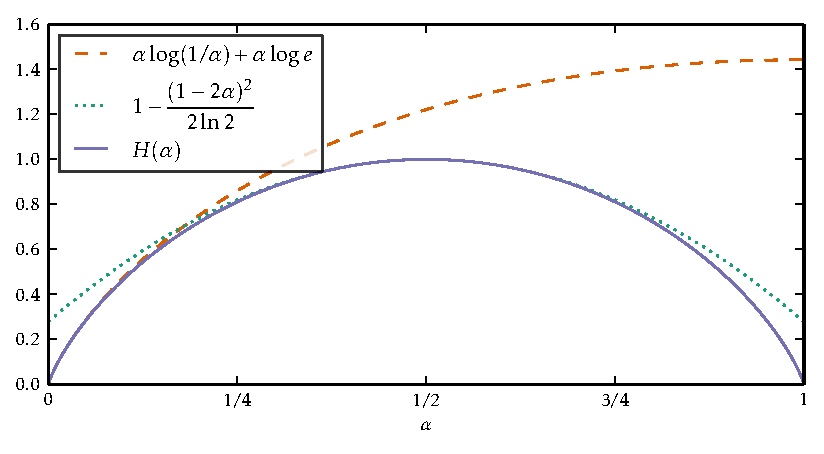
\includegraphics{entropy}}
  \caption{Binary entropy, $H$, and two useful approximations.}
  \figlabel{entropy}
\end{figure}

Notice that we have already encountered a quantity that can be
expressed in terms of the binary entropy.  From
\eqref{sparse-bitstring-ii}, a bit string of length $n$ that has
exactly $k$ one bits can be encoded with a fixed length code of length
$nH(k/n)$.

The binary entropy function can be difficult to work with, so it is
helpful to have some manageable approximations.  One of these is
derived as follows:
\begin{align}
  H(\alpha) & = \alpha\log(1/\alpha) + (1-\alpha)\log(1/(1-\alpha)) \notag \\
            & = \alpha\log(1/\alpha) + (1-\alpha)\log(1+\alpha/(1-\alpha)) \notag \\
            & \le \alpha\log(1/\alpha) + \alpha\log e \eqlabel{entropy-i} 
\end{align}
since $1+x\le e^x$ for all $x\in\mathbb{R}$. \Eqref{entropy-i} is a
useful approximation when $\alpha$ is close to zero, so that
$H(\alpha)$ is also close to zero.

For $\alpha$ close to $1/2$ (so that $H(\alpha)$ is close to 1), we
obtain a good approximation from the Taylor series expansion at
$1/2$. In particular, for $\alpha=(1-\eps)/2$,
\begin{align}
  H(\alpha) & = 1-\frac{1}{2\ln 2}\sum_{i=1}^{\infty}\frac{(1-2\alpha)^{2i}}{i(2i-1)} 
              \notag \\ 
            & = 1-\frac{1}{2\ln 2}\sum_{i=1}^{\infty}\frac{\eps^{2i}}{i(2i-1)} 
              \notag \\ 
            & < 1-\frac{\eps^2}{2\ln 2} \enspace .\eqlabel{entropy-ii}
\end{align}

\subsection{Basic Chernoff Bound}

Since we now have the pieces we need, we give an encoding argument for
a well-known and extremely useful result typically attributed to
Chernoff \cite{chernoff:bound}.

\begin{thm}\thmlabel{chernoff-basic}
  Let $x\in\{0,1\}^n$ be chosen uniformly at random.Then
  \[
    \Pr\{n_1(x) \le n(1-\eps)/2\} < e^{-\eps^2n/2} \enspace .
  \]
\end{thm}

\begin{proof}
  Encode the bit string $x$ using a Shannon-Fano code, $C_\alpha$,
  with $\alpha=(1-\eps)/2$.  Then the length of the codeword for $x$
  is
  \[
    |C_\alpha(x)| = n_1(x)\log(1/\alpha) + n_0(x)\log (1/(1-\alpha))
    \enspace .
  \]
  Since $\alpha < 1/2$, $\log(1/\alpha) > \log(1/(1-\alpha))$, so
  $|C_\alpha(x)|$ is maximal when $n_1(x)$ is maximal.  Under the
  conditions of the theorem, this happens when $n_1(x)=\alpha n$.
  Therefore,
  \begin{align*}
    |C_\alpha(x)| & \le \alpha n\log(1/\alpha) + (1-\alpha)n\log(1/(1-\alpha))\\
                  & = n H(\alpha) \\
                  & \le n\left(1-\frac{\eps^2}{2\ln 2}\right) \enspace ,
  \end{align*}
  where the second inequality is an application of \eqref{entropy-ii}.
  Now, $x$ was chosen uniformly at random from a set of size $2^n$.
  Therefore, this encoding saves:
  \[  
    s = n-\left(n\left(1-\frac{\eps^2}{2\ln 2}\right)\right) =
    \frac{\eps^2n}{2\ln 2}
  \]
  bits.  By the Uniform Encoding Lemma, the probability that this
  happens is at most
  \[
    2^{-s} = e^{-\eps^2n/2} \enspace . \qedhere
  \]
\end{proof}
In \secref{chernoff}, after developing a Non-Uniform Encoding Lemma,
we will extend this argument to binary strings where each bit is set
independently to 1 or 0 with probabilities $p$ and $1-p$,
respectively.

\subsection{Factorials and Binomial Coefficients}
\seclabel{stirling}

Before moving on to some more advanced encoding arguments, it will be
helpful to remind the reader of a few inequalities that can be derived
from Stirling's Approximation of $n!$.  Recall that Stirling's
Approximation states that
\begin{equation}
  n! = \left(\frac{n}{e}\right)^n\sqrt{2\pi n}\left(1+\Theta\left(\frac{1}{n}\right)\right) \enspace .
  \eqlabel{stirling}
\end{equation}

In many cases, we are interested in representing a set of size $n!$
using a fixed-length code.  The length of the codewords in such a code
is
\begin{align}
  \log n!
  & = n\log n - n\log e + (1/2)\log n + \log \sqrt{2 \pi} + \log(1+\Theta(1/n)) \notag \\
  & = n\log n - n\log e + (1/2)\log n + \log \sqrt{2 \pi} + \Theta(1/n) \notag \\
  & = n\log n - n\log e + \Theta(\log n) \eqlabel{stirling-loose}
    \enspace .
\end{align}

We are sometimes interested in codes for the $\binom{n}{k}$ subsets of
$k$ elements from a set of size $n$. Note that there is an easy
bijection between such subsets and binary strings of length $n$ having
exactly $k$ ones. Therefore, we can represent these using the
Shannon-Fano code $C_{k/n}$ and each of our codewords will have length
$nH(k/n)$.  In particular, this implies that
\begin{equation}
  \log\binom{n}{k} \le nH(k/n) \le k\log n - k\log k + k\log e 
  \eqlabel{log-n-choose-k}
\end{equation}
where the last inequality is an application of \eqref{entropy-i}. The
astute reader will notice that we just used an encoding argument to
prove an upper-bound on $\binom{n}{k}$ \emph{without knowing the formula $\binom{n}{k}=\frac{n!}{k! (n - k)!}$}. Alternatively, we could obtain
a slightly worse bound by applying 
\eqref{stirling} to this formula.

\subsection{Encoding the Natural Numbers}

We have so far only explicitly been concerned with codes for finite
sets. In this section, we give an outline of the design of some
prefix-free codes for the set of natural numbers. Of course, if $p :
\N \to [0, 1]$ is a probability density, then the Shannon-Fano code
for $p$ could serve. However, it seems easier to simply design our
codes by hand, rather than find appropriate distributions.

A code is prefix-free if and only if any message consisting of a
sequence of its codewords can be decoded unambiguously as it is read
from left to right. This idea allows us to more easily design the
codes in this section, which were originally given by
Elias~\cite{elias:coding}.

The \emph{unary encoding} of an integer $i \in \N$ begins with $i$ 1
bits which are punctuated with a 0 bit. This code is not particularly
useful in itself. The \emph{Elias $\gamma$-code} for $i$ begins with
the unary encoding of the number of bits in $i$, and then the binary
encoding of $i$ itself (minus its leading bit). The \emph{Elias
  $\delta$-code} for $i$ begins with an Elias $\gamma$-code for the
number of bits in $i$, and then the binary encoding of $i$ itself
(minus its leading bit). This process can be continued recursively to
obtain the \emph{Elias $\omega$-code}.

The most important properties of these codes are their codeword
lengths:
\begin{align*}
  |U(i)| &= i + 1 \enspace , \tag{Unary code} \\
  |E_\gamma(i)| &= 2 \log i + O(1) \enspace , \tag{Elias $\gamma$-code} \\
  |E_\delta(i)| &= \log i + 2 \log \log i + O(1) \enspace , \tag{Elias $\delta$-code} \\
  |E_\omega(i)| &= \log i + \log \log i + \dots + \underbrace{\log \cdots \log}_{\text{$\log^* i$ times}}i + O(\log^* i) \enspace . \tag{Elias $\omega$-code}
\end{align*}
It may be worth noting that the lengths of Elias $\gamma$-codes
correspond to the lengths of Shannon-Fano codes for a discrete Cauchy
distribution.

\section{Applications of the Uniform Encoding Lemma}
\seclabel{applications-i}

We now start with some applications of the Uniform Encoding Lemma. In
each case, we will design and analyze a partial prefix-free code
$C\from X\nrightarrow \{0, 1\}^*$, where $X$ is to be understood from
the context.

\subsection{Graphs with no Large Clique or Independent Set}

The \emph{Erd\H{o}s-R\'enyi random graph} $G_{n,p}$ is the space of
graphs with vertex set $V=\{1,\ldots,n\}$ and in which each edge $\{u,
w\} \in \binom{V}{2}$ is present with probability $p$ and absent with
probability $1-p$, independently of the other edges.  Erd\H{o}s
\cite{erdos:some} used the random graph $G_{n,\frac{1}{2}}$ to prove
the existence of graphs having no large clique and no large
independent set. Here we show how this can be done using an encoding
argument.

\begin{thm}\thmlabel{erdos-renyi-i}
  For $n \ge 3$, the probability that $G \in G_{n,\frac{1}{2}}$
  contains a clique or an independent set of size $t = \ceil{3\log n +
    \sqrt{2s}}$ is at most $2^{-s}$.
\end{thm}

\begin{proof}
  This is an encoding argument that compresses the $\binom{n}{2}$ bits
  of $G$'s adjacency matrix, as they appear in row-major order.
  
  The graph $G$ contains a clique or independent set $S$ of size
  $t$. Hence, the code $C(G)$ begins with a bit indicating whether $S$
  is a clique or independent set; the set of vertices of $S$; then the
  adjacency matrix of $G$ in row major-order but leaving out all of
  the $\binom{t}{2}$ bits implied by the edges or non-edges in $S$.
  
  Such a codeword has length
  \begin{align*}
    |C(G)| & = 1 + t\log n + \binom{n}{2}-\binom{t}{2} \\
    & = \binom{n}{2} + 1 + t\log n - (1/2)(t^2 - t) \\
    & = \binom{n}{2} + 1 - (1/2)(t^2 - t - 2t \log n) \enspace .
  \end{align*}
  The function $f(x) = (1/2)(x^2 - x - 2x \log n) - 1$ is increasing
  for $x \geq \log n + 1/2$, so
  \begin{align*}
    f(t) &\ge f(3\log n + \sqrt{2s}) \\
    &= (1/2)(9 \log^2 n + 6 \sqrt{2s} \log n + 2s - 3 \log n - \sqrt{2s} - 6 \log^2 n - 2 \sqrt{2s} \log n) - 1 \\
    &= (1/2)(3 \log^2 n + 4 \sqrt{2s} \log n - 3 \log n - \sqrt{2s}) + s - 1 \\
    &\ge s
  \end{align*}
  for $n \ge 3$. Therefore, our code has length
  \begin{align*}
    |C(G)| & = \binom{n}{2} - f(t) \\
    & \le \binom{n}{2} - s \enspace .
  \end{align*}
  Applying the Uniform Encoding Lemma completes the proof.
\end{proof}

\begin{rem}
  The bound in \thmref{erdos-renyi-i} can be strengthened a little,
  since the elements of $S$ can be encoded using only
  $\log\binom{n}{t}$ bits, rather than $t\log n$.  With a more careful
  calculation, using \eqref{log-n-choose-k}, the proof then works with
  $t = 2\log n +O(\log\log n) + \sqrt{s}$. This comes closer to Erdős'
  original result, which was at the threshold $2\log n - 2\log\log n +
  O(1)$.
\end{rem}


\subsection{Balls in Urns}
\seclabel{urns}

The question of what happens when one throws $n$ balls uniformly and
independently at random into $n$ urns is a useful abstraction of many
algorithmic, data structures, and load-balancing problem.  Here we
show how an encoding argument can be used to prove the classic result
that, when we do this, no urn contains more than $O(\log n/\log\log
n)$ balls.

\begin{thm}\thmlabel{urns}
  Let $t$ be such that $t\log(t/e) \ge s+\log n$ and suppose we throw
  $n$ balls independently and uniformly at random into $n$ urns. Then,
  for sufficiently large $n$, the probability that any urn contains
  more than $t$ balls is at most $2^{-s}$.
\end{thm}

Before proving \thmref{urns}, we note that, for any constant $\eps >0$
and all sufficiently large $n$, taking
\[
  t = \Ceil{\frac{(1+\eps)\log n}{\log\log n}}
\] 
satisfies the requirements of \thmref{urns}.

\begin{proof}
  For each $i\in\{1,\ldots,n\}$, let $b_i$ denote the index of the urn
  in which the $i$\textsuperscript{th} ball lands. Notice that the
  sequence $b = (b_1,\ldots,b_n)$ is chosen uniformly at random from a
  set of size $n^n$, and it is this choice that will be used in our
  encoding argument.

  If the urn labelled $i$ contains $t$ or more balls, then our code
  begins with the value $i$, followed by a code that describes $t$ of
  the balls in urn $i$, followed by the remaining $n-t$ values of
  $b_1,\ldots,b_n$ that cannot be deduced from the preceding
  information.  In total, this is
  \begin{align*}
    |C(b)| &= \log n + \log\binom{n}{t} + (n-t)\log n \\
           &= \log n + t\log n - t\log t + t\log e + (n-t)\log n
             \tag{using \eqref{log-n-choose-k}} \\
           & = n \log n + \log n - t\log t + t\log e \\
           & \le n \log n - s \tag{by the choice of $t$} \\
           & = \log n^n - s
  \end{align*}
  bits. We conclude the proof by applying the Uniform Encoding Lemma.
\end{proof}

\subsection{Linear Probing}

Studying balls in urns is a useful technique to analyze hashing with
chaining (see \emph{e.g.}~\cite[Section~5.1]{morin:open}). A more
practically efficient form of hashing is \emph{linear probing}.  In a
linear probing hash table, we hash the elements $x_1, \ldots, x_n$
into a hash table of size $m=cn$, for some fixed $c> 1$. We are given
a hash function $h : \{x_1, \ldots, x_n\} \to \{1, \ldots, m\}$ which
we assume to be a uniform random variable. To insert $x_i$, we try and
place it at table position $j=h(x_i)$, unless it is already occupied
by one of $x_1,\ldots,x_{i-1}$, in which case we try table location
$(j+1)\bmod m$, $(j+2)\bmod m$, and so on until we find an empty spot
for $x_i$.  We want to study the expected search time for some item
$x_i$ in this hash table.

We call a maximal consecutive sequence of occupied table locations a
\emph{block}. The table locations $m-1$ and $0$ are considered
consecutive.

\begin{thm}\thmlabel{linear-probing}
  Fix some $x\in\{x_1,\ldots,x_n\}$. Then the probability that the
  block containing $x$ has size at least $t$, for $t$ satisfying
  \[
    t \log (c/e) - \log t \ge s + O(1) \enspace ,
  \]
  is at most $2^{-s}$.
\end{thm}

\begin{proof}
  This is an encoding argument that encodes the function $h$ by
  encoding the sequence
  \[
    (h(x_1),h(x_2),\ldots,h(x_n)) \enspace ,
  \]
  which is drawn uniformly at random from a set of size
  $n^{m}=n^{cn}$.
  
  We encode $h$ by the first index $b$ of the block containing $x$;
  followed by the $t-1$ elements $y_1,\ldots,y_{t-1}$ of this block
  (excluding $x$); followed by enough information to decode the hash
  values of $h(x)$ and $h(y_1),\ldots,h(y_{t-1})$; followed by
  $h(x_1),\ldots,h(x_n)$ excluding the $t$ hash values we can compute
  from the preceding information.

  Notice that $h(x),h(y_1),h(y_2),\ldots,h(y_{t-1})$ are in the range
  $b,\ldots,b+t-1$ (modulo $m$) so these can be encoded using
  $t\log t$ bits.  Therefore, if the block containing $x$ has size
  $t$, then we obtain a codeword whose length is
  \begin{align*}
    |C(h)| & = \overbrace{\log m}^{b} + \overbrace{\log\binom{n}{t-1}}^{y_1,\ldots,y_{t-1}} + \overbrace{t\log t}^{h(x),h(y_1),\ldots,h(y_{t-1})} + \overbrace{(n-t)\log m}^{\text{everything else}} \\
           & \le \log m + (t-1)\log n - 
             (t-1)\log(t-1) + (t-1)\log e + t\log t + (n-t)\log m \tag{by \eqref{log-n-choose-k}}\\
           & \le \log m + (t-1)\log n + (t-1)\log e + (n-t)\log m + \log t+ O(1)\\
           & = n\log m - (t-1)\log c + (t-1)\log e + \log t + O(1) \tag{since $m = cn$}\\
           & = \log m^n - (t-1)\log(c/e) + \log t + O(1) \\
           & \le \log m^n - s \enspace ,
  \end{align*}
  for all $t$ satisfying
  \[
    t \log (c/e) - \log t \ge s + O(1) \enspace .
  \]
  The proof is complete by applying the Uniform Encoding Lemma.
\end{proof}

\begin{rem}
  The proof of \thmref{linear-probing} requires that the linear
  probing hash table has size $cn$ for some $c>e$.  We know from
  previous analysis that this is not necessary, and any $c>1$ is
  sufficient. We leave it as an open problem to find an encoding proof
  of \thmref{linear-probing} that works for any $c>1$.
\end{rem}

\begin{cor}
  A linear probing hash table of size $cn$ with $c > e$ achieves
  $O(1)$ expected search time.
\end{cor}
\begin{proof}
  Let $S$ denote the size of the largest block in such a hash
  table. From \thmref{linear-probing}, any fixed $x_i$ is contained in
  a block of size at least $2s/\log (c/e) + s_0$ with probability at
  most $2^{-s}$, for some constant $s_0$. Then,
  \begin{align*}
    \E\{S\} &= \sum_{s = 1}^\infty \Pr\{S \ge s\} = \sum_{i=1}^{s_0} \Pr\{S \ge s\} + \sum_{s = 1}^\infty \Pr\{S \ge s + s_0\} \\
            &\le s_0 + \sum_{s = 1}^\infty 2^{-s \log (c/e)/2} = s_0 + \sum_{s = 1}^\infty (c/e)^{-s/2} = O(1) \enspace . \qedhere
  \end{align*}
\end{proof}

\subsection{Cuckoo Hashing}

Cuckoo hashing is relatively new kind of hash table that offers an
alternative to classic perfect hashing \cite{pagh.rodler:cuckoo}. Here
we present a clever proof, due to Mihai Pătraşcu, that cuckoo hashing
succeeds with probability $1-O(1/n)$ \cite{patrascu:cuckoo}.

%The main object of study in cuckoo hashing is the \emph{cuckoo graph},
%a random bipartite multigraph $G=(A,B,E)$ where $|A|=|B|=m$ for $m =
%2n$, and $|E|=n$.  For each $i\in\{1,\ldots,n\}$, each edge $e_i$ of
%$E$ is obtained by randomly choosing (with replacement) an endpoint
%$a_i\in A$ and an endpoint $b_i\in B$.  The cuckoo hashing algorithm
%may fail if this graph contains a long edge-simple path or if it
%contains a component with more edges than vertices.  (An edge-simple
%path is a path that uses each edge of the multiset $E$ at most once.)

We again hash the elements $x_1, \ldots, x_n$. The hash table consists
of two arrays $A$ and $B$ of size $m = 2n$, and two hash functions $h,
g : \{x_1, \ldots, x_n\} \to \{1, \ldots, m\}$ which are uniform
random variables. To insert an element $x$ into the hash table, we
insert it into $A[h(x)]$; if $A[h(x)]$ already contains an element
$y$, we insert $y$ into $B[g(y)]$; if $B[g(y)]$ already contains some
element $z$, we insert $z$ into $A[h(z)]$, etc. If an empty location
is eventually found, the algorithm terminates successfully. If a cycle
is detected, then the hash table is rebuilt using different hash
functions. Any element $x$ either is held in $A[h(x)]$ or $B[g(x)]$,
so we can search for $x$ in constant time.

To study the performance of insertion in cuckoo hashing, we study the
random bipartite \emph{cuckoo graph} $G = (A, B, E)$, where $|A| = |B|
= m$ and $|E| = n$, with each vertex corresponding either to a
location in the array $A$ or $B$ above, and with edge multiset $E =
\{(h(x_i), g(x_i)) : 1 \leq i \leq n\}$.

An edge-simple path is a path which uses each edge at most once. Such
a path in this graph describes the potential motion of elements in a
hash table insertion. Thus, in bounding the length of edge-simple
paths in the cuckoo graph, we bound the worst case insertion time.

\begin{lem}\lemlabel{cuckoo-path-length}
  The cuckoo graph has an edge-simple path of length at least
  $s + \log n + O(1)$ with probability at most $2^{-s}$.
\end{lem}
\begin{proof}
  We encode $G$ by presenting its set of edges. Since each endpoint of
  an edge is chosen independently and uniformly at random from a set
  of size $n$, then the set of all edges is chosen uniformly at random
  from a set of size $m^{2n}$.

  Suppose that some vertex $v$ is the endpoint of an edge-simple path
  of length $t$; such a path has $t + 1$ vertices and $t$ edges. In
  the encoding, we present the $t$ edges of the path in order; then,
  we indicate whether $v \in A$ or $v \in B$; and we give the $t + 1$
  vertices in order starting from $v$; and finally, the remaining
  $2n - 2t$ endpoints of edges of the graph. This code has length
  \begin{align*}
    |C(G)| &= t \log n + 1 + (t + 1) \log m + (2n - 2t) \log m\\
           &= 2n \log m + t \log n - t \log m + \log m + O(1) \\
           &= \log m^{2n} - t + \log n + O(1) \tag{since $m = 2n$} \\
           &\leq \log m^{2n} - s
  \end{align*}
  for $t \geq s + \log n + O(1)$. We finish by applying the Uniform
  Encoding Lemma.
\end{proof}
This immediately implies that a successful insertion takes time at
most $2 \log n + O(1)$ with probability $1 - O(1/n)$.

The cuckoo hashing insertion algorithm can fail if some subgraph of
the cuckoo graph contains more edges than vertices, since edges
correspond to keys, and vertices correspond to array locations.
\begin{lem}\lemlabel{cuckoo-failure}
  The cuckoo graph has a subgraph with more edges than vertices with
  probability $O(1/n)$. In other words, cuckoo hashing succeeds with
  probability $1 - O(1/n)$.
\end{lem}
\begin{proof}
  Suppose that some vertex $v$ is part of a subgraph with more edges
  than vertices, and in particular a minimal such subgraph with $t +
  1$ edges and $t$ vertices. Such a subgraph appears exactly as in
  \figref{cuckoo-cycles}. For every such subgraph, there are two edges
  $e_1$ and $e_2$ whose removal disconnects the graph into two paths
  of length $t_1$ and $t_2$ starting from $v$, where $t_1 + t_2 = t -
  1$.

  \begin{figure}
    \centering
    \begin{subfigure}[b]{0.3\textwidth}
      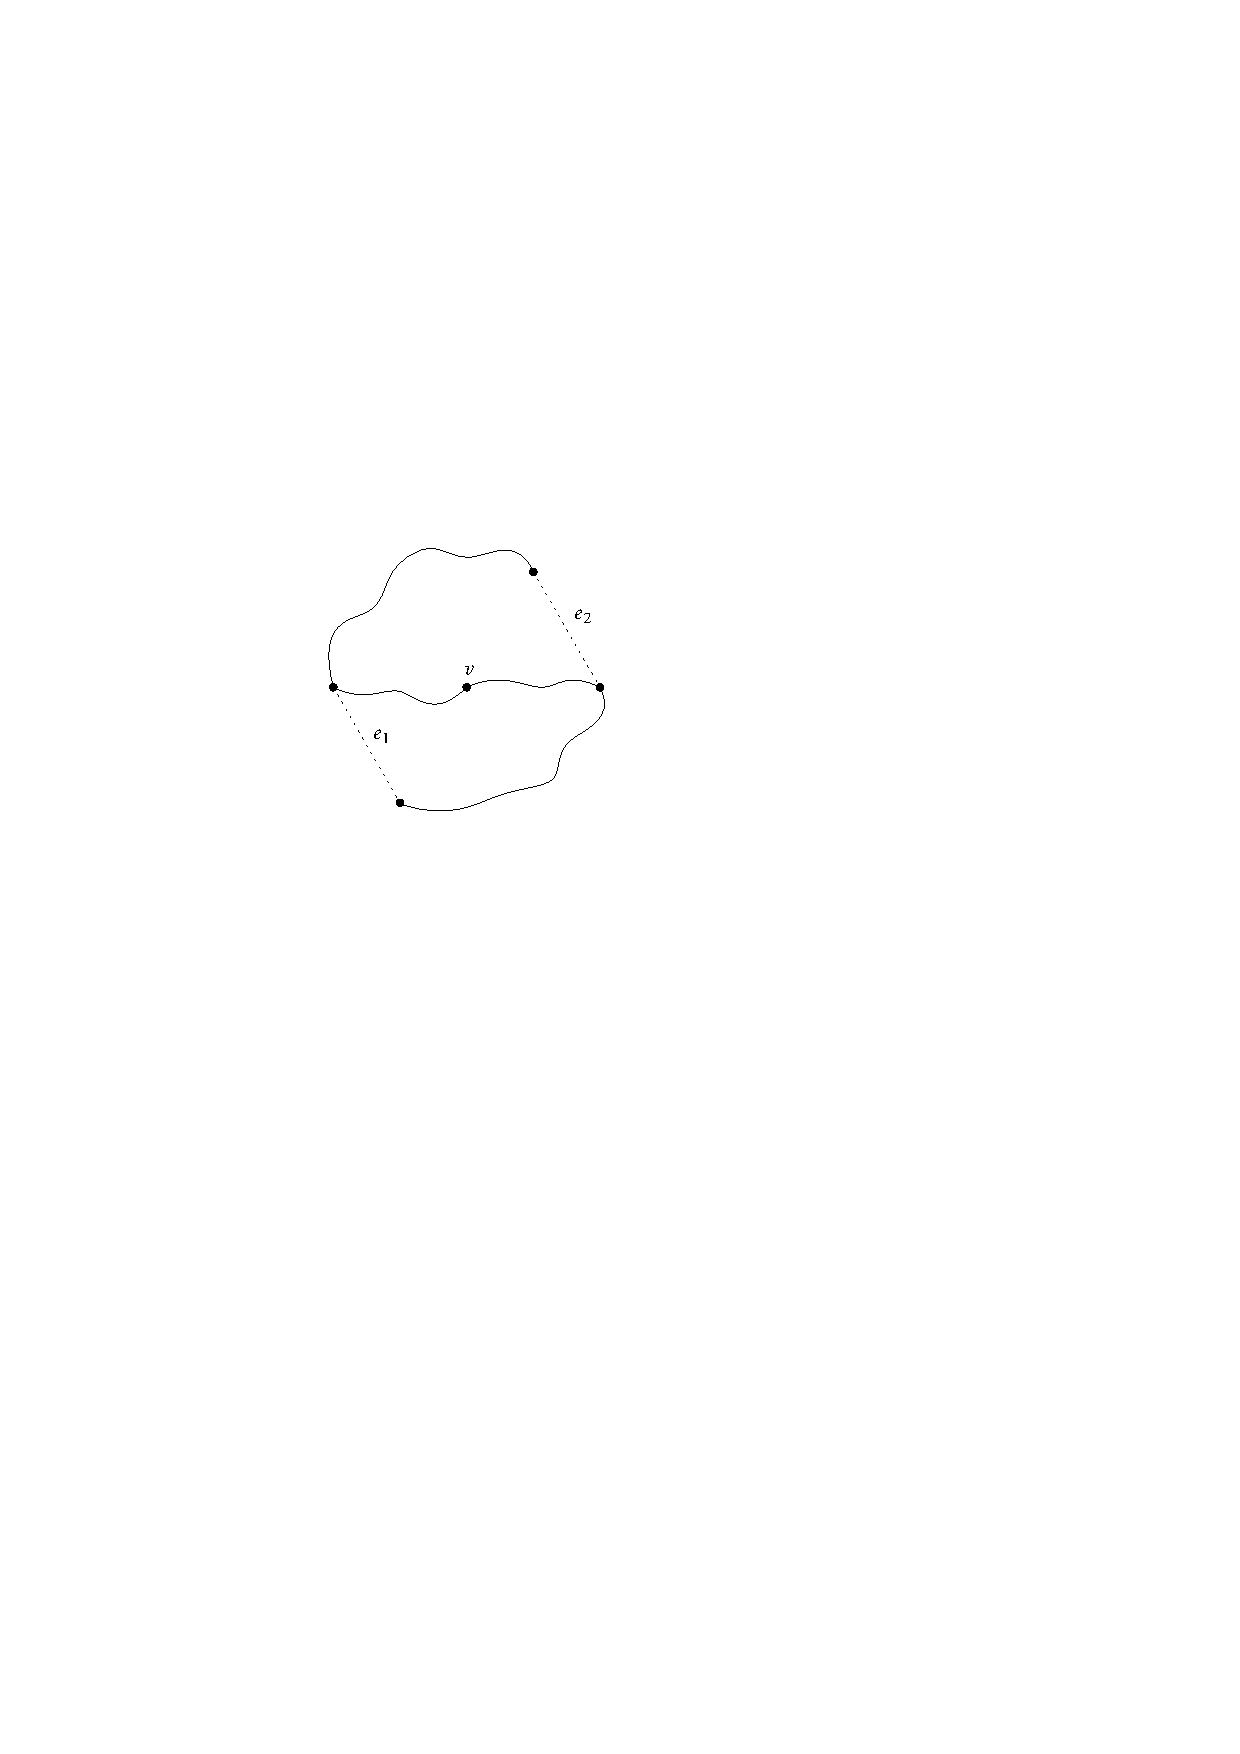
\includegraphics{cuckoo1}
      \caption{A cycle with a chord.}
    \end{subfigure}
    \quad\quad
    \begin{subfigure}[b]{0.6\textwidth}
      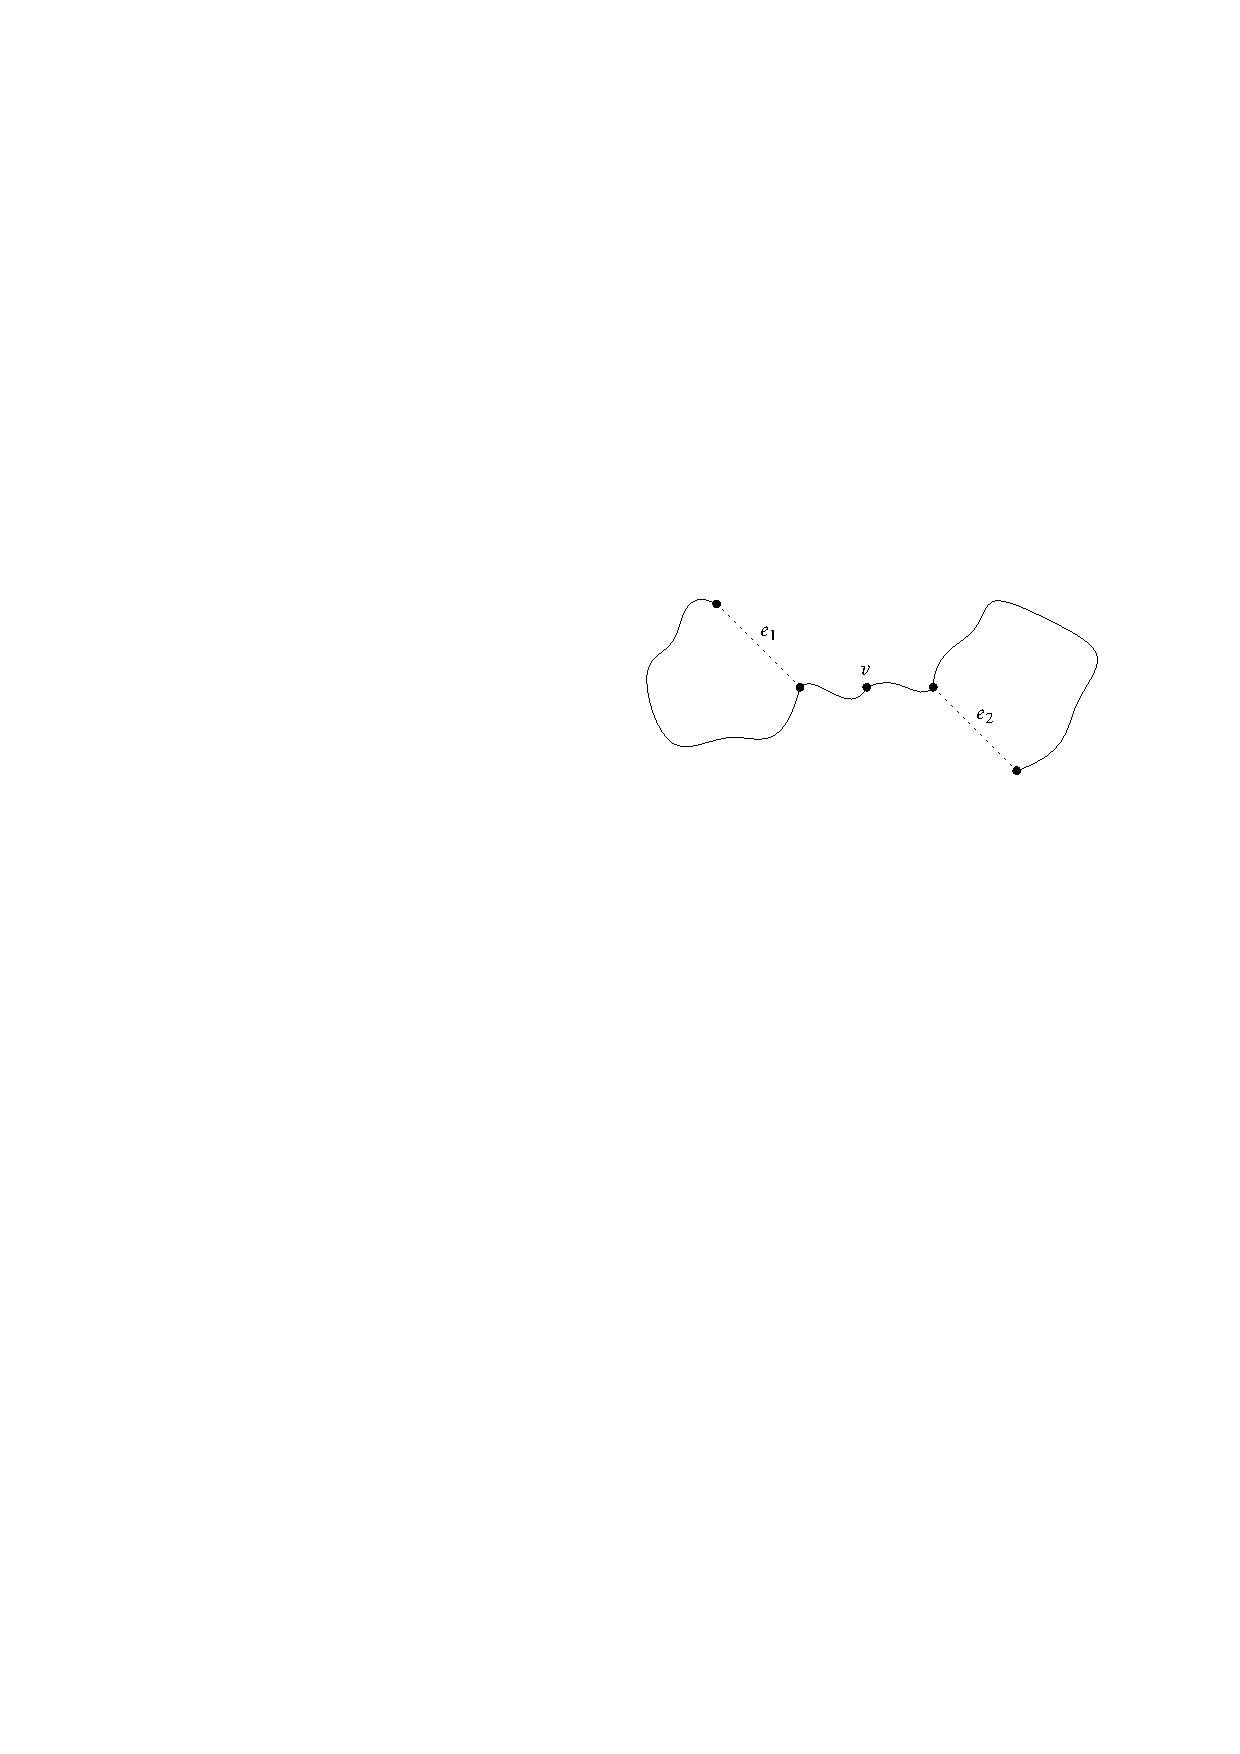
\includegraphics{cuckoo2}
      \caption{Two cycles connected by a path.}
    \end{subfigure}
    \caption{The potential minimal subgraphs of the cuckoo graph.}
    \figlabel{cuckoo-cycles}
  \end{figure}

  We encode $G$ by giving the vertex $v$; and presenting Elias
  $\delta$-codes for the values of $t_1$ and $t_2$; then the edges of
  the above paths in order; then the vertices of the paths in order;
  and the edges $e_1$ and $e_2$; and finally the remaining $2n - 2(t +
  1)$ endpoints of edges in the graph. Such a code has length
  \begin{align*}
    |C(G)| &= \log n + (t - 1)(\log n + \log m) + 2\log n + (2n - 2(t + 1))\log m + O(\log t) \\
           &= 2n \log m + \log n - 2\log m - t + O(\log t) \\
           &\leq \log m^{2n} - \log n + O(1) \enspace .
  \end{align*}
  We finish by applying the Uniform Encoding Lemma.
\end{proof}

\subsection{2-Choice Hashing}

We showed in \secref{urns} that if $n$ balls are thrown independently
and uniformly at random into $n$ urns, then the maximum number of
balls in any urn is $O(\log n/\log \log n)$ with high probability. In
\emph{2-choice hashing}, each ball is instead given a choice of two
urns, and the urn containing the fewer balls is preferred.

More specifically, we are given two hash functions $h, g : X \to \{1,
\ldots, m\}$ which are uniform random variables. Each value of $h$ and
$g$ points to one of $m$ urns. The element $x \in X$ is added to the
urn containing the fewest elements between $h(x)$ and $g(x)$ during an
insertion. The worst case search time is at most the maximum number of
hashing collisions, or the maximum number of elements in any urn.

Perhaps surprisingly, the simple change of having two choices instead
of only one results in an exponential improvement over the strategy of
\secref{urns}. 2-choice hashing was first studied by Azar \emph{et
  al.}~\cite{azar:multiplechoice}, who showed that the expected
maximum size of an urn is $\log \log n + O(1)$. Our encoding argument
is based on V\"{o}cking's use of witness trees to analyze 2-choice
hashing~\cite{vocking:witness}.

Let $G = (V, E)$ be the random multigraph with $V = \{1, \ldots, m\}$,
where $m = cn$ for some constant $c > 4$, and
$E = \{(h(x), g(x)) : x \in X\}$.

\begin{lem}\lemlabel{two-choice-two-cycles}
  $G$ has a subgraph with more edges than vertices with probability
  $O(1/n)$.
\end{lem}
\begin{proof}
  The proof is similar to that of \lemref{cuckoo-failure}. More
  specifically, we can encode $G$ by giving the same encoding as in
  \lemref{cuckoo-failure}, with an additional bit for each edge $uv$
  in the encoding, indicating whether $u = h(x)$ and $v = g(x)$, or $u
  = g(x)$ and $v = h(x)$. Our code thus has length
  \begin{align*}
    |C(G)| &= \log n + (t - 1)(\log n + \log m) + 2 \log n + (2n - 2(t + 1))\log m + t + O(\log t) \\
           &= 2n \log m - \log n - t \log c + t + O(\log t) \\
           &\le \log m^{2n} - \log n + O(1) \enspace ,
  \end{align*}
  since $\log c > 1$.
\end{proof}

\begin{lem}\lemlabel{two-choice-component-size}
  $G$ has a component of size at least $(2/\log(c/4))\log n + O(1)$
  with probability $O(1/n)$.
\end{lem}
\begin{proof}
  Suppose $G$ has a connected component with $t - 1$ edges and at most
  $t$ vertices. This component has a spanning tree $T$. Pick an
  arbitrary vertex as the root of $T$. We encode $G$ by specifying
  first the $t - 1$ edges and $t$ vertices encountered in a pre-order
  traversal of $T$; then a bit string encoding the shape of $T$; and
  finally the remaining $2(n - t + 1)$ endpoints of edges.

  We can encode the shape of $T$ using a bit string of length
  $2(t - 1)$, tracing a pre-order traversal of the tree, where a 0 bit
  indicates that the path to the next node goes up, and a 1 indicates
  that the path goes down. In total, our code has length
  \begin{align*}
    |C(G)| &= t \log m + (t - 1) \log n + 2(t - 1) + 2 (n - t + 1) \log m \\
           &= 2n\log m + t \log c - \log n + 2t - 2 - 2t \log c + 2\log n + 2 \log c \tag{since $m = cn$}\\
           &= \log m^{2n} - t \log c + 2t + \log n + O(1) \\
           &\le \log m^{2n} - s \enspace ,
  \end{align*}
  as long as $t$ is such that
  \[
    t \geq \frac{s + \log n + O(1)}{\log (c/4)} \enspace .
  \]
  In particular, if we choose $s = \log n$, applying the Uniform
  Encoding Lemma tells us that $G$ has a component of size at least
  $(2/\log (c/4))\log n + O(1)$ with probability $O(1/n)$.
\end{proof}

Suppose that when $x$ is inserted, it is placed in a urn with $t$
other elements. Then, we say that the age of $x$ is $a(x) = t$.
\begin{thm}
  The cost of searching in 2-choice hashing in a table of size $cn$
  with $c > 4$ is at most $\log \log n + O(1)$ with probability $1 -
  O(1/n)$.
\end{thm}
\begin{proof}
  Suppose that some element $x$ has $a(x) = t$. This leads to a binary
  \emph{witness tree} $T$ of height $t$ as follows: The root of $T$ is
  the element $x$. When $x$ was inserted into the hash table, it had
  to choose between the urns $h(x)$ and $g(x)$, both of which
  contained at least $t - 1$ elements; in particular, $h(x)$ has an
  element $x_h$ with $a(x_h) = t - 1$, and $g(x)$ has an element $x_g$
  with $a(x_g) = t - 1$. The elements $x_h$ and $x_g$ become left and
  right children of $x$ in $T$. The process continues recursively. If
  some element appears more than once on a level, we only recurse on
  its leftmost occurence. Note that each vertex of $T$ corresponds to
  the edge $(h(x), g(x))$ of $G$. Moreover, the subgraph of $G$
  induced by the edges
  \[
    \{(h(x), g(x)) : x \text{ is a vertex of } T\}
  \]
  is connected.

  Suppose that some node appears more than once on a level of
  $T$. From above, this means that some component of $G$ has a
  cycle. If this happens twice, then $G$ has a subgraph with more
  edges than vertices. By \lemref{two-choice-two-cycles}, this happens
  with probability $O(1/n)$. If instead this happens at most once,
  then $T$ has at most one subtree removed, so $T$ has at least $2^t$
  nodes. If we choose $t = \ceil{\log \log n + d}$, then $T$ has at
  least $2^d \log n$ nodes, which we know from
  \lemref{two-choice-component-size} happens with probability $O(1/n)$
  for a sufficiently large choice of the constant $d$.
\end{proof}

\begin{rem}
  The arguments in this section can be refined by more carefully
  encoding the shape of trees using Cayley's formula. In particular, a
  rooted tree with $t$ nodes and $m$ choices for distinct node labels
  can be encoded using $\log \binom{m}{t} + (t - 2) \log t$ bits
  instead of $t \log m + 2(t - 1)$ bits. We would then recover the
  same results for hash tables of size $m = cn$ for $c > e$ instead of
  $c > 4$. In fact, it suffices that $c > 0$ for searching to take
  time $O(\log \log n)$ in 2-choice hashing. We leave it as an open
  problem to find an encoding argument for this result when $c > 0$.
\end{rem}

\begin{rem}
  Robin Hood hashing is another hashing solution which achieves
  $O(\log \log n)$ worst case running time for all
  operations~\cite{devroye:robin}. The original analysis is difficult,
  but might lend itself to a similar kind of analysis as we used in
  this section. Indeed, when a Robin Hood hashing operation takes a
  significant amount of time, a large witness tree is again implied,
  which suggests an easy encoding argument. Unfortunately, this
  approach appears to involve unwieldy hypergraph encoding.
\end{rem}


\subsection{Bipartite Expanders}

Expanders are families of graphs which share some isoperimetric
quality, \emph{i.e.}~where subgraphs ``expand'' in their
neighbourhoods. These graphs have received much research attention,
and have been shown to have many applications in computer
science. See, for instance, the survey by Hoory, Linial, and
Wigderson~\cite{hoory.linial.ea:expander}.

We offer an encoding argument to prove that a certain random bipartite
graph is an expander with high probability. There are many different
notions of expansion. We will consider what is commonly known as
vertex expansion in bipartite graphs: For some fixed $0 < \alpha \leq
1$, a bipartite graph $G = (A, B, E)$ is called a \emph{$(c,
  \alpha)$-expander} if
\begin{align*}
  \min_{\substack{{A' \subseteq A}\\{|A'| \leq \alpha |A|}}} \frac{|N(A')|}{|A'|} \geq c \enspace ,
\end{align*}
where $N(A') \subseteq B$ is the set of neighbours of $A'$ in $G$.

Let $G = (A, B, E)$ be a random bipartite multigraph where $|A| = |B|
= n$ and where each vertex of $A$ is connected to three vertices of
$B$ chosen independently and uniformly at random (with
replacement). The following theorem shows that $G$ is an expander.
The proof of this theorem usually involves a messy sum that contains
binomial coefficients and probabilities: see, for example, Motwani and
Raghavan~\cite[Theorem~5.3]{motwani.raghavan:randomized},
Pinsker~\cite[Lemma~1]{pinsker:on}, or Hoory, Linial, and
Wigderson~\cite[Lemma~1.9]{hoory.linial.ea:expander}.

\begin{thm}
  There exists a constant $\alpha >0$ such that $G$ is a
  $(3/2,\alpha)$-expander with probability at least $1 - O(n^{-1/2})$.
\end{thm}

\begin{proof}
  We encode the graph $G$ by presenting its edge set. Since each edge
  is selected uniformly at random, then $G$ is chosen uniformly at
  random from a set of size $n^{3n}$.
  
  If $G$ is not a $(3/2, \alpha)$-expander, then there is some set $A'
  \subseteq A$ with $|A'|=k\le \alpha n$ and
  \[
  \frac{|N(A')|}{|A'|} < 3/2 \enspace .
  \]
  To encode $G$, we first give $k$ using an Elias $\gamma$-code; and
  we give the sets $A'$ and $N(A')$; and the edges between $A'$ and
  $N(A')$. Then we encode the rest of $G$, skipping the $3k\log n$
  bits devoted to elements in $A'$.  The key savings here come because
  $N(A')$ should take $3k\log n$ bits to encode, but can actually be
  encoded in roughly $3k\log(3k/2)$ bits. Our code then has length
  \begin{align*}
    |C(G)| &= 2\log k + \log {n \choose k} + \log {n \choose 3k/2} + 3k \log (3k/2) + (3n - 3k)\log n + O(1) \\
           &\leq 3n \log n - (k/2)\log n + (k/2)\log k + \beta k + 2 \log k + O(1) \tag{by \eqref{log-n-choose-k}}\\
           &= \log n^{3n} - s(k)
  \end{align*}
  bits, where $\beta = (3/2) \log (3/2) + (5/2) \log e$. Note that
  \[
    \frac{d^2}{dk^2} s(k) = \frac{4 - k}{2 k^2} \log e \enspace ,
  \]
  so that $s(k)$ is concave for all $k \geq 4$. Thus, $s(k)$ is
  minimized either when $k = 1, 2, 3, 4$, or $k = \alpha n$. We have
  \begin{align*}
    s(1) &= (1/2)\log n + c_1 \enspace , & 
    s(2) &= \log n + c_2 \enspace , \\
    s(3) &= (3/2) \log n + c_3 \enspace , &
    s(4) &= 2 \log n + c_4 \enspace ,
  \end{align*}
  for constants $c_1, c_2, c_3, c_4$. For $k=\alpha n$ we have
  \[
    s(\alpha n) = (\alpha n/2)\log \left(\frac{1}{2^{2\beta}
        \alpha}\right) - 2 \log \alpha n
  \]
  and $2^{-s(\alpha n)} = 2^{-\Omega(n)}$ for
  $\alpha < (1/2)^{2\beta} \approx 0.002$. In each case, the Uniform
  Encoding Lemma gives the desired result, and in particular,
  $2^{-s(k)} \leq O(n^{-1/2})$.
\end{proof}

\subsection{Permutations and Binary Search Trees}

A \emph{permutation} $\sigma$ of size $n$ is a sequence of $n$
distinct integers, sometimes denoted
$\sigma = (\sigma_1, \ldots, \sigma_n)$. Except when explicitly
stated, we will assume that the set of integers involved in a
permutation of size $n$ is precisely $\{1, \ldots, n\}$. The number of
such permutations is $n!$.

\subsubsection{Analysis of Insertion Sort}
\seclabel{insertion-sort}

Recall the insertion-sort algorithm for sorting a list
$\sigma = (\sigma_1,\ldots,\sigma_n)$ of $n$ elements:

\noindent{$\textsc{InsertionSort}(\sigma)$}
\begin{algorithmic}[1]
  \FOR{$i\gets 2$ \TO $n$}
     \STATE{$j \gets i$}
     \WHILE{$j>1$ \AND $x_{j-1} > x_j$}
         \STATE{$\sigma_j \leftrightarrow \sigma_{j-1}$
            \COMMENT{ swap }}
         \STATE{$j\gets j-1$}
     \ENDWHILE
  \ENDFOR
\end{algorithmic}

A typical question asks the expected number of times Line~4 executes
if $\sigma$ is a uniformly random permutation of size $n$.  The answer
$\binom{n}{2}/2$ is an easy application of linearity of expectation:
For every one of the $\binom{n}{2}$ pairs $p,q\in\{1,\ldots,n\}$ with
$p<q$, the values initially stored at positions $\sigma_p$ and
$\sigma_q$ will eventually be swapped if and only if
$\sigma_p > \sigma_q$, which happens with probability $1/2$ in a
uniformly random permutation.

A more advanced question is to ask for a concentration result on the
number of executions of Line~4. This is a harder question to tackle;
because $>$ is transitive, the $\binom{n}{2}$ events being studied
have a lot of interdependence. In the following, we show how to obtain
a concentration result with an encoding argument.  The argument
presented here follows the same outline as Vit\'{a}nyi's analysis of
bubble sort \cite{vitanyi:analysis}, though without all the trappings
of Kolmogorov complexity.

\begin{thm}\thmlabel{insertion-sort}
  For a uniformly random permutation $\sigma$ of size $n$, the
  probability that Line~4 of $\textsc{InsertionSort}(\sigma)$ executes
  fewer than $\alpha n^2 - n + 2$ times is at most $2^{n\log(\alpha
    e^2)+O(\log n)}$.  In particular, for a fixed $\alpha < 1/e^2$,
  this probability is $2^{-\Omega(n)}$.
\end{thm}

\begin{proof}
  %Let $\sigma$ be the permutation of $\{1,\ldots,n\}$ that defines the
  %sorted order of $x_1,\ldots,x_n$, so that $x_{\sigma(j)}$ is the
  %element that appears at position $j$ after sorting. Notice that
  %$\sigma$ is chosen uniformly at random among all $n!$ permutations
  %of of $\{1,\ldots,n\}$.
  %
  We encode the permutation $\sigma$ by recording the execution of
  \textsc{InsertionSort} on this permutation. In particular, we record
  for each $i\in\{2,\ldots,n\}$, the number of times $m_i$ that Line~4
  executes during the $i$\textsuperscript{th} iteration of
  $\textsc{InsertionSort}(\sigma)$. With this information, one can run
  the following algorithm to recover $\sigma$:
  
  \noindent{$\textsc{InsertionSortReconstruct}(m_2,\ldots,m_n)$}:
  \begin{algorithmic}[1]
    \STATE{$\sigma \gets (1,\ldots,n)$}
    \FOR{$i\gets 2$ \TO $n$}
       \FOR{$j\gets i \textbf{ down to } i-m_i+1$}
           \STATE{$\sigma_j \leftrightarrow \sigma_{j-1}$
              \COMMENT{ swap }}
       \ENDFOR
    \ENDFOR
    \RETURN{$\sigma$}
  \end{algorithmic}
   
  To make this work, we have to be slightly clever with this
  encoding. Rather than encode $m_2,m_3,\ldots,m_n$ directly, we first
  encode $m=\sum_{i=2}^{n} m_i$ using $2\log n$ bits (since
  $m < n^2$). Given $m$, what remains is to describe the partition of
  $m$ into $n-1$ non-negative integers $m_2,\ldots,m_n$; there are
  $\binom{m+n-2}{n-2}$ such partitions.\footnote{To see this, draw
    $m+n-2$ white dots on a line, then choose $n-2$ dots to colour
    black. This splits the remaining $m$ white dots up into $n-1$
    groups, which determine the values of $m_2,\ldots,m_n$.}
  
  Therefore, the values of $m_2,\ldots,m_n$ can be encoded using
  \[
    |C(\sigma)| = 2\log n + \log\binom{m+n-2}{n-2}
  \]
  bits and this is sufficient to recover the permutation $\sigma$.  By
  applying \eqref{log-n-choose-k}, we obtain
  \begin{align*}
    |C(\sigma)| & \le (n-2)\log(m+n-2) - (n-2)\log(n-2)  + (n-2)\log e + O(\log n) \\
      & \le n\log(m+n-2) - n\log n   + n\log e + O(\log n) \\
      & \le n\log(\alpha n^2) - n\log n  + n\log e + O(\log n) \\
      & = 2n\log n + n\log\alpha - n\log n  + n\log e + O(\log n) \\
      & = n\log n + n\log\alpha + n\log e + O(\log n) \\
      & = \log n! + n\log\alpha + 2n\log e + O(\log n) \tag{by \eqref{stirling-loose}} \\
      & = \log n! + n \log (\alpha e^2) + O(\log n) \enspace .
  \end{align*}
  Again, we finish by applying the Uniform Encoding Lemma.
\end{proof}


\begin{rem}
  Although it doesn't require any advanced probability,
  \thmref{insertion-sort} is not sharp; it only gives a non-trivial
  probability when $\alpha < 1/e^2$.  To obtain a sharp bound, one can
  use the fact that $m_2,\ldots,m_n$ are independent and $m_i$ is
  uniform over $\{0,\ldots,i-1\}$ and then use the method of bounded
  differences \cite{mcdiarmid:on} to show that $m$ is concentrated in
  an interval of size $O(n^{3/2})$.
\end{rem}

\subsubsection{Records}

A \emph{(max) record} in a permutation $\sigma$ of size $n$ is some
value $\sigma_i$ with $1 \leq i \leq n$ such that
\[
  \sigma_i = \max\{\sigma_1, \dots, \sigma_i\} \enspace .
\]
It is easy to see that the probability that $\sigma_i$ is a record is
exactly $1/i$ if $\sigma$ is chosen uniformly at random, in which case
the expected number of records in such a permutation is
\[
  H_n = \sum_{i = 1}^n 1/i = \ln n + O(1) \enspace ,
\]
the $n$\textsuperscript{th} harmonic number. It is harder to establish
concentration with non-negligible probability. To do this, one first
needs to show the independence of certain random variables, which
quickly becomes tedious. We instead give an encoding argument to show
concentration of the number of records, inspired by a technique used
by Lucier \emph{et al.} to study the height of random binary search
trees \cite{lucier.jiang.li:quicksort}.

First, we describe an incremental and recursive manner of encoding a
permutation $\sigma$ of size $n$: Begin by providing the first value
of the permutation $\sigma_1$; followed by the set of indices of the
permutation for which $\sigma$ takes on a value strictly smaller than
$\sigma_1$, including an explicit encoding of the induced permutation
on the elements at those indices; and a recursive encoding of the
permutation induced on the elements strictly larger than $\sigma_1$.

If $\sigma$ contains $k$ elements strictly smaller than $\sigma_1$,
then the length $\ell(n)$ of the codeword for $\sigma$ satisfies the
recurrence
\[
  \ell(n) = \log n + \log \binom{n - 1}{k} + \log k! + \ell(n - k - 1) \enspace ,
\]
with $\ell(0) = 0$ and $\ell(1) = 0$. This solves to $\ell(n) = \log
n!$, so the encoding described above is no better than a fixed-length
encoding for $\sigma$. However, we can readily modify this encoding to
obtain a result about the concentration of records in a uniformly
random permutation.

\begin{thm}\thmlabel{records}
  A uniformly random permutation $\sigma$ of size $n$ has at least $c
  \log n$ records with probability at most
  \[
    2^{-c (1 - H(1/c)) \log n + O(\log \log n)}
  \]
  for $c > 2$.
\end{thm}
\begin{proof}
  We encode the permutation $\sigma$ chosen uniformly at random from a
  set of size $n!$.

  Suppose that $\sigma$ has $t = \ceil{c\log n}$ records
  $r_1 < r_2 < \cdots < r_t$, for some fixed $c > 2$. First, give a
  bit string $x = (x_1, \dots, x_t) \in \{0, 1\}^t$, where $x_i = 0$
  if and only if $r_i$ lies in the first half of the interval
  $[r_{i - 1}, n]$. It follows that $n_1(x) \leq \log n$, so
  $n_1(x)/t \leq 1/c$.

  To begin our encoding of $\sigma$, we encode the bit string $x$ by
  giving the set of $n_1(x)$ ones in $x$; followed by the incremental
  recursive encoding of $\sigma$ from earlier. Now, our knowledge of
  the value of $x_i$ halves the size of the space of options for
  encoding the record $r_i$. In other words, our knowledge of $x$
  allows us to encode each record using roughly one less bit per
  record. More precisely, if the number of choices for each record
  $r_i$ in the original encoding is $m_i$, such that $m_1 > \dots >
  m_t$, then the number of bits spent encoding records in the new code
  is at most
  \begin{align*}
    \sum_{i = 1}^t \log \ceil{m_i/2} &\leq \sum_{i = 1}^t \log (m_i/2
    + 1)
    \leq \sum_{i = 1}^t \log (m_i/2) + \sum_{i = 1}^t O(1/m_i) \\
    &\leq \sum_{i = 1}^t \log (m_i/2) + O(H_t) = \sum_{i = 1}^t \log
    m_i - t + O(\log \log n) \enspace .
  \end{align*}
  Thus, the total length of the code is
  \begin{align*}
    |C(\sigma)| &\leq \binom{t}{n_1(x)} + \log n! - t + O(\log \log n) \\
                &\leq \log n! - t (1 - H(n_1(x)/t)) + O(\log \log n) \tag{by \eqref{log-n-choose-k}}\\
                &\leq \log n! - c (1 - H(1/c))\log n + O(\log \log n) \enspace ,
  \end{align*}
  where this last inequality follows since $c > 2$, so $H(n_1(x)/t)
  \leq H(1/c)$. We finish by applying the Uniform Encoding Lemma.
\end{proof}

\begin{rem}\remlabel{records}
  The preceding result only works for $c > 2$, but we already know
  that the number of records in a uniformly random permutation is
  concentrated around $\ln n + O(1)$, where $\ln n = \alpha \log n$
  for $\alpha = 0.6931...$. We leave as an open problem whether or not
  this significant gap can be closed through an encoding argument.
\end{rem}

\subsubsection{The Height of a Random Binary Search Tree}
\seclabel{height}

Every permutation $\sigma$ determines a binary search tree
$\text{BST}(\sigma)$ created through the sequential insertion of the
keys $\sigma_1, \ldots, \sigma_n$. Specifically, if $\sigma^L$
(respectively, $\sigma^R$) denotes the permutation of elements
strictly smaller (respectively, strictly larger) than $\sigma_1$, then
$\text{BST}(\sigma)$ has $\sigma_1$ as its root, with
$\text{BST}(\sigma^L)$ and $\text{BST}(\sigma^R)$ as left and right
subtrees.

Lucier \emph{et al.}~\cite{lucier.jiang.li:quicksort} use an encoding
argument via Kolmogorov complexity to study the height of
$\text{BST}(\sigma)$. They show that for a uniformly chosen
permutation $\sigma$, the tree $\text{BST}(\sigma)$ has height at most
$c \log n$ with probability $1 - O(1/n)$ for $c = 15.498...$; we can
extend our result on records to obtain a tighter result.

For a node $u$, let $s(u)$ denote the number of nodes in the tree
rooted at $u$. Then, $u$ is called \emph{balanced} if $s(u^L), s(u^R)
> s(u)/4$, where $u^L$ and $u^R$ are the left and right subtrees of
$u$ respectively. In other words, a node is said to be balanced if it
occurs in the middle half of its subrange.

\begin{thm}\thmlabel{bst-height}
  Let $\sigma$ be a uniformly random permutation of size $n$. Then,
  $\text{BST}(\sigma)$ has height $O(\log n)$ with high probability.
\end{thm}
\begin{proof}
  Suppose that the tree $\text{BST}(\sigma)$ has a root-to-leaf path
  $Y = (y_1, \ldots, y_t)$ of length $t = \ceil{c \log n}$ for some
  fixed $c > 2/\log (4/3)$.

  Our encoding for $\sigma$ has two parts. The first part includes an
  encoding of the value $y_t$, and a bit string
  $x = (x_1, \ldots, x_t)$, where $x_i = 1$ if and only if $y_i$ is
  balanced. From our definition, if $y_i$ is balanced, then
  $s(y_{i + 1}) \leq (3/4) s(y_i)$, and since $n_1(x)$ counts the
  number of balanced nodes along $Y$, then
  \[
    1 \leq (3/4)^{n_1(x)} n \iff n_1(x) \leq \log_{4/3} n \enspace .
  \]

  The second part of our encoding is recursive: First, encode the
  value of the root $r$ using $\log \ceil{n/2}$ bits. If the
  path $Y$ goes to the left of $r$, then specify the values in the
  right subtree of $r$, including an explicit encoding of the
  permutation induced by these values; and recursively encode the
  permutation of values in the left subtree of $r$. If, instead, $Y$
  goes to the right of $r$, we proceed symmetrically.
 
  The first part of our encoding uses at most
  \[
    \log n + t H(n_1(x)/t)
  \]
  bits. The same analysis as performed in \thmref{records} shows that
  the second part of our encoding has length at most
  \[
    \log n! - t + O(\log \log n) \enspace .
  \]
  Applying the Uniform Encoding Lemma, we see that
  $\text{BST}(\sigma)$ has height at most $c \log n$ with probability
  $1 - O(1/n)$ for $c > 2/\log (4/3)$ satisfying
  \[
    c \left(1 - H\left(\frac{1}{c \log (4/3)}\right)\right) > 1 \enspace ,
  \]
  and a computer-aided calculation shows that $c = 8.12669...$ is the
  minimal solution so this inequality.
\end{proof}

\begin{rem}
  Devroye~\cite{devroye:records} shows how the length of the path to
  the key $i$ in $\text{BST}(\sigma)$ relates to the number of records
  in $\sigma$. Specifically, he notes that the number of records in
  $\sigma$ is the number of nodes along the rightmost path in
  $\text{BST}(\sigma)$. Since the height of a tree is the length of
  its longest root-to-leaf path, we obtain as a corollary that the
  number of records in a uniformly random permutation is $O(\log n)$
  with high probability; the result from \thmref{records} only
  improves upon the implied constant.
\end{rem}

\begin{rem}
  We know that the height of the binary search tree built from the
  sequential insertion of elements from a uniformly random permutation
  of size $n$ is concentrated around $\alpha \ln n + O(\log \log n)$,
  for $\alpha = 4.311...$~\cite{reed:height}. Perhaps if the gap in
  our analysis of records in \remref{records} can be closed through an
  encoding argument, then so too can the gap in our analysis of random
  binary search tree height.
\end{rem}

\subsubsection{Hoare's Find Algorithm}

In this section, we analyze the number of comparisons made in the
execution of Hoare's classic \textsc{Find} algorithm~\cite{hoare:find}
which returns the $k$\textsuperscript{th} smallest element in an array
of $n$ elements. The analysis is similar to that of the preceding
section.

We assume knowledge of the algorithm $\textsc{Partition}$, which takes
as input an array $\sigma = (\sigma_1, \dots, \sigma_n)$ and
partitions it into the arrays $\sigma^L$ and $\sigma^R$ which contain
the values strictly smaller and strictly larger than $\sigma_1$,
respectively. The element $\sigma_1$ is called a \emph{pivot}. It is
easy to see how $\textsc{Partition}$ can be implemented so as to
perform only $n - 1$ comparisons. The algorithm $\textsc{Find}$ is
then implemented as follows:

\noindent{$\textsc{Find}(k, \sigma)$}:
\begin{algorithmic}[1]
  \STATE{$\sigma^L, \sigma^R \gets \textsc{Partition}(\sigma)$}
  \IF{$|\sigma^L| \geq k$}
    \RETURN{$\textsc{Find}(k, \sigma^L)$}
  \ELSIF{$|\sigma^L| < k - 1$}
    \RETURN{$\textsc{Find}(k - |\sigma^L| - 1, \sigma^R)$}
  \ENDIF
  \RETURN{$\sigma_k$}
\end{algorithmic}

As the algorithm executes, it sequentially identifies $k$ pivots $x_1,
\dots, x_k$ before finding the solution. We will say that a pivot is
\emph{good} if it lies in the interval $[n/4, 3n/4]$. Note that a good
pivot causes the algorithm to recurse in a problem of size at most
$3n/4$.

\begin{lem}
  Fix some constants $k_0 \geq 1$ and $0 < \alpha < 1/2$. Suppose
  that, for each $k_0 \leq i \leq k$, the number of good pivots among
  $x_1, \ldots, x_i$ is at least $\alpha i$. Then, $\textsc{Find}$
  makes $O(n)$ comparisons.
\end{lem}
\begin{proof}
  Let $m_i$ be the size of the input array during the
  $i$\textsuperscript{th} recursive call, and in particular $m_0 =
  n$. If $x_j$ is a good pivot, then the conditions of the lemma give
  that $m_j \le (3/4) m_{j - 1}$. Therefore,
  \[
  m_i \leq (3/4)^{\alpha i} n
  \]
  for each $k_0 \leq i \leq k$, and the total number of comparisons
  made by $\textsc{Find}$ is at most
  \[
  \sum_{i=0}^k (m_i + 1) \le k_0(n + 1) + k + \sum_{i=k_0}^k m_i \le
  O(n) + n \sum_{i = k_0}^k (3/4)^{\alpha i} = O(n) \enspace . \qedhere
  \]
\end{proof}

\begin{thm}
  For a uniformly random permutation $\sigma$ and any $k$,
  $\textsc{Find}(k, \sigma)$ executes $O(n)$ comparisons with high
  probability.
\end{thm}
\begin{proof}
  We again encode the permutation $\sigma$. Suppose that the
  conditions of the preceding lemma are not satisfied,
  \emph{i.e.}~there is an $i$ such that the number of good pivots
  among $x_1, \dots, x_i$ is less than $\alpha i$. We encode $\sigma$
  in two parts. The first part of our encoding gives the value of $i$
  using an Elias $\delta$-code, followed by the set of indices of the
  good pivots among $x_1, \dots, x_i$, which costs
  \[
  \log i + i H(\alpha) + O(\log \log i) \enspace .
  \]
  Note that the pivots $x_1, \dots, x_i$ trace a path from the root in
  $\text{BST}(\sigma)$. Therefore, the second part of our encoding is
  the recursive encoding presented in \secref{height}, in which each
  pivot can be encoded using one less bit. In total, our code then has
  length
  \[
    |C(\sigma)| \le \log n! - i + i H(\alpha) + \log i + O(\log \log
    i) = \log n! - \Omega(i) \enspace ,
  \]
  since $\alpha < 1/2$. The proof is completed by applying the Uniform
  Encoding Lemma, and by observing that $k_0 \leq i$ can be made
  arbitrarily large.
\end{proof}


\subsection{$k$-SAT and the Lov\'{a}sz Local Lemma}

A \emph{variable} $x$ is either $\textsf{true}$ or
$\textsf{false}$. The negation of $x$ is denoted by $\neg x$. A
\emph{literal} is either a variable or its negation. A
\emph{conjunction} of literals is an ``and'' of literals, denoted by
$\land$. A \emph{disjunction} of literals is an ``or'' of literals,
denoted by $\lor$. A \emph{formula} $\varphi$ is an expression
including conjunctions and disjunctions of literals, and the set of
variables involved in this formula is called the \emph{support} of
$\varphi$. A \emph{clause} is a disjunction of literals, \emph{i.e.}
the ``or'' of a set of variables or their negations, \emph{e.g.}
\begin{align}
  x_1 \lor \neg x_2 \lor x_3 \enspace . \eqlabel{clause-example}
\end{align}
Two clauses will be said to intersect if their supports intersect. The
truth value which a formula $\varphi$ evaluates to under the
assignment of values $\alpha$ to its support will be denoted
$\varphi(\alpha)$, and such a formula is said to be \emph{satisfiable}
if $\varphi(\alpha) = \textsf{true}$ for some $\alpha$. For example,
the clause in \eqref{clause-example} is satisfied for all truth
assignments except
\[
(x_1, x_2, x_3) = (\textsf{false}, \textsf{true}, \textsf{false}) \enspace ,
\]
and indeed any clause is satisfied by any but one truth assignment for
its support. The formulas we are concerned with are conjunctions of
clauses, which are said to be in \emph{conjunctive normal form}
(CNF). More specifically, when each clause has $k$ literals, we call
it a $k$-CNF formula.

The $k$-SAT decision problem asks to determine whether or not a given
$k$-CNF formula is satisfiable. In general, this problem is hard. Of
course, any satisfiable truth assignment to the variables in a CNF
formula induces a truth assignment for each of its clauses; the
converse is true if each clause is pairwise disjoint, and as we will
see, even if each clause is only nearly pairwise disjoint, \emph{i.e.}
their intersection has size less than $2^k/e$.

This result has been well known as a consequence of the Lov\'{a}sz
Local Lemma~\cite{lovasz:locallemma}, whose original proof is
non-constructive, and so would not produce a satisfying truth
assignment as applied to an instance of $k$-SAT. Some constructive
solutions to $k$-SAT have been known, but only for suboptimal clause
intersection sizes. Moser and Tardos~\cite{moser:locallemma} famously
presented the first constructive proof of the full Lov\'{a}sz Local
Lemma, which also gives a construction for $k$-SAT. The analysis which
we reproduce in this section comes from Fortnow's rephrasing of
Moser's proof for $k$-SAT using the incompressibility
method~\cite{fortnow:ksat}.

Moser's algorithm is remarkably naive, and can be described in only a
few sentences: Pick a uniformly random truth assignment for the
variables of $\varphi$. For each unsatisfied clause, attempt to fix it
by producing a new uniformly random truth assignment for its support,
and recursively fix any intersecting clause which is made unsatisfied
by this reassignment. We describe this process more carefully in the
algorithms $\textsc{Solve}$ and $\textsc{Fix}$ below.

\noindent{$\textsc{Solve}(\varphi)$}:
\begin{algorithmic}[1]
  \STATE{$\alpha \gets $ uniformly random truth assignment in $\{\textsf{true}, \textsf{false}\}^n$}
  \WHILE{$\varphi(\alpha) = \textsf{false}$}
    \STATE{$D \gets $ an unsatisfied clause in $\varphi$}
    \STATE{$\alpha \gets \textsc{Fix}(\varphi, \alpha, D)$}
  \ENDWHILE
  \RETURN{$\alpha$}
\end{algorithmic}

\noindent{$\textsc{Fix}(\varphi, \alpha, D)$}:
\begin{algorithmic}[1]
  \STATE{$\beta \gets $ uniformly random truth assignment in $\{\textsf{true}, \textsf{false}\}^k$}
  \STATE{replace the assignments in $\alpha$ for $D's$ support with the values in $\beta$}
  \WHILE{$\varphi(\alpha) = \textsf{false}$}
    \STATE{$D' \gets $ an unsatisfied clause in $\varphi$ intersecting $D$}
    \STATE{$\alpha \gets \textsc{Fix}(\varphi, \alpha, D')$}
  \ENDWHILE
  \RETURN{$\alpha$}
\end{algorithmic}

\begin{thm}
%  Let $a \in \{\textsf{true}, \textsf{false}\}^n$ and $b_i \in
%  \{\textsf{true}, \textsf{false}\}^{k}$ for each $1 \le i \le s$ be
%  chosen uniformly at random.
%
  Given a $k$-CNF formula $\varphi$ with $m$ clauses and $n$ variables
  such that each clause intersects at most $r \le 2^{k - 3}$ other
  clauses, the probability that $\textsc{Solve}(\varphi)$ calls
  $\textsc{Fix}$ at least $s + m \log m$ times is at most $2^{-s}$.
\end{thm}
\begin{proof}
  Suppose that $\textsc{Solve}(\varphi)$ calls $\textsc{Fix}$
  $t = \ceil{s + m\log m}$ times. Let
  $\alpha \in \{\textsf{true}, \textsf{false}\}^n$ be the initial
  truth assignment for $\varphi$, and let
  $\beta_1, \ldots, \beta_t \in \{\textsf{true}, \textsf{false}\}^k$
  be the local truth assignments produced in each call to
  $\textsc{Fix}$. The string
  $\gamma = (\alpha, \beta_1, \ldots, \beta_t)$ is uniformly chosen
  from a set of size $2^{n + tk}$, and will be the subject of our
  encoding.

  The execution of $\textsc{Solve}(\varphi)$ determines a (rooted
  ordered) \emph{recursion tree} $T$ on $t + 1$ nodes as follows: The
  root of $T$ corresponds to the initial call to
  $\textsc{Solve}(\varphi)$, and its children $D_1, \ldots, D_d$
  recursively correspond to the sequence of calls to
  $\textsc{Fix}(\varphi, \alpha, D_1), \ldots, \textsc{Fix}(\varphi,
  \alpha, D_d)$. In particular, each (non-root) node in the tree is
  assigned a clause and its uniformly random truth assignment produced
  during the call to $\textsc{Fix}$. Moreover, a pre-order traversal
  of this tree describes the order of function calls in the
  algorithm's execution.

  The string $\gamma$ can be recovered from the bottom-up from our
  knowledge of the tree $T$ and the final assignment
  $\alpha$. Specifically, let $D_1, \dots, D_t$ be the clauses
  encountered in a pre-order traversal of $T$, so that in particular
  $D_t$ is the last fixed clause in the execution. Since $D_t$ was not
  satisfied before its reassignment, this allows us to deduce $k$
  values of $\alpha$ before $D_t$ was fixed. Pruning $D_t$ from the
  tree and continuing in this manner at $D_{t - 1}$, we eventually
  recover the original truth assignment produced in
  $\textsc{Solve}(\varphi)$.

  Therefore, to encode $\gamma$, we first give the final truth
  assignment $\alpha$; and a description of the shape of the tree $T$;
  and the sequence of at most $m$ clauses which are children of the
  root of $T$; and the at most $t$ clauses involved in the calls to
  $\textsc{Fix}$ in a pre-order traversal of $T$.

  The key savings come from the fact that each clause intersects at
  most $r$ other clauses, so each clause (which is not a child of the
  root) can be encoded using $\log r$ bits. Each clause which is a
  child of the root can be encoded using $\log m$ bits, and since the
  order of these children might be significant, we use $m \log m$ bits
  to encode the full sequence of these clauses. Finally, as in
  \lemref{two-choice-component-size}, the shape of $T$ can be encoded
  using $2t$ bits. In total, the code has length
  \begin{align*}
    |C(\gamma)| &\le n + 2t + m\log m+ t \log r \\
    &\le n + 2t + m\log m + t(k - 3) \tag{since $r \le 2^{k - 3}$} \\
    &= n + tk - t + m\log m \\
    &\le n + tk - s \enspace .
  \end{align*}
  The result is obtained by applying the Uniform Encoding Lemma.
\end{proof}

\begin{rem}
  By more carefully encoding of the shape of the recursion tree above,
  Messner and Thierauf~\cite{messner:ksat} gave an encoding argument
  for the above result in which $r < 2^k/e$. Their refinement follows
  from a more careful counting of the number of trees with nodes of
  bounded degree.
\end{rem}

\section{The Non-Uniform Encoding Lemma and Shannon-Fano Codes}
\seclabel{nuel}

Thus far, we have been lucky to study applications that could always
be modelled as choosing some element $x$ uniformly at random from a
set $X$. To encompass even more applications, it is helpful to have an
Encoding Lemma that deals with non-uniform distributions over
$X$. First, recall the following useful classic results:
\begin{thm}[Markov's Inequality]
  For any non-negative random variable $X$ with finite expectation,
  and any $a > 0$,
  \[
    \Pr\{X \geq a\} \leq (1/a) \E\{X\} \enspace .
  \]
\end{thm}

We will say that a real-valued function $\ell : X \to \R$
\emph{satisfies Kraft's condition} if
\[
  \sum_{x \in X} 2^{-\ell(x)} \leq 1 \enspace .
\]
\begin{lem}[Kraft's Inequality]
  If $C : X \nrightarrow \{0,1\}^*$ is a partial prefix-free code,
  then $|C(\cdot)|$ satisfies Kraft's condition. Conversely, for any
  function $\ell : X \to \N$ satisfying Kraft's condition, there
  exists a prefix-free code $C : X \to \{0, 1\}^*$ such that
  $|C(x)| = \ell(x)$ for all $x \in X$.
\end{lem}

The following generalization of the Uniform Encoding Lemma, which was
originally proven by Barron~\cite[Theorem~3.1]{barron:dissertation},
serves for non-uniform input distributions:
\begin{lem}[Non-Uniform Encoding Lemma]\lemlabel{nuel}  
  Let $C\from X\nrightarrow\{0,1\}^*$ be a partial prefix-free code
  and let $x\in X$ be drawn randomly where $p_x$ denotes the
  probability of drawing $x$.  Then
  \[
    \Pr\{ |C(x)| \le \log(1/p_x)-s\} \le 2^{-s} \enspace .
  \]
\end{lem}

\begin{proof}
  We use Chernoff's trick, Markov's inequality, and Kraft's
  inequality, as follows:
  \begin{align*}
    \Pr\{ |C(x)| \le\log(1/p_x)-s \}
    & = \Pr\{|C(x)| -\log(1/p_x) \le -s \} \\
    & = \Pr\{\log(1/p_x)-|C(x)| \ge s \} \\
    & = \Pr\left\{2^{\log(1/p_x)-|C(x)|} \ge 2^s \right\}  \tag{Chernoff's trick} \\
    & \le \frac{\E\left\{2^{\log(1/p_x)-|C(x)|}\right\}}{2^s} \tag{Markov's inequality} \\
    & = \frac{1}{2^s} \left(\sum_{x\in X : C(x) \neq \bot} p_x\cdot 2^{\log(1/p_x)-|C(x)|}\right) \\
    & = \frac{1}{2^s} \left(\sum_{x\in X : C(x) \neq \bot }2^{-|C(x)|}\right) \enspace .
  \end{align*}
  By Kraft's inequality,
  $\sum_{x \in X : C(x) \neq \bot} 2^{-|C(x)|} \leq 1$, and the result
  is obtained.
\end{proof}

Notice that the Non-Uniform Encoding Lemma is a strict generalization
of the Uniform Encoding Lemma: Take $p_x=1/|X|$ for all $x\in X$ and
we obtain the Uniform Encoding Lemma.

As in \secref{sparse-bit-strings}, we will be interested in using a
Shannon-Fano code $C_\alpha$ to encode $\mathrm{Bernoulli}(\alpha)$
bit strings of length $n$. Recall that for such a string $x$, this
code has length
\[
  n_1(x) \log (1/\alpha) + n_0(x) \log(1/(1 - \alpha)) \enspace ,
\]
since we are not concerned with ceilings.

\section{Applications of the Non-Uniform Encoding Lemma}
\seclabel{applications-ii}

\subsection{Chernoff Bound}
\seclabel{chernoff}

We will now prove the so-called \emph{additive version} of the
Chernoff bound on the tail of a binomial random
variable~\cite{chernoff:bound}. \thmref{chernoff-basic} established
the special case of this result for $\mathrm{Bernoulli}(1/2)$ bit
strings.

\begin{thm}\thmlabel{chernoff}
  If $B$ is a $\mathrm{Binomial}(n,p)$ random variable, then
  \[
    \Pr\{B\le(p-\eps)n\} \le 2^{-nD(p-\eps \| p)} \enspace ,
  \]
  where 
  \[ 
    D(p \| q)= p\log (p/q) + (1-p)\log ((1 - p)/(1 - q))
  \]
  is the \emph{Kullback-Liebler divergence} or \emph{relative entropy}
  between $\mathrm{Bernoulli}(p)$ and $\mathrm{Bernoulli}(q)$ random
  variables.
\end{thm}

\begin{proof}
  By definition, $B=\sum_{i=1}^n x_i$, where $x_1,\ldots,x_n$ are
  independent $\mathrm{Bernoulli}(p)$ random variables.  We will use
  an encoding argument on the bit string $x=(x_1,\ldots,x_n)$. The
  proof is almost identical to that of \thmref{chernoff-basic}---now,
  we encode $x$ using a Shannon-Fano code $C_\alpha$, with
  $\alpha = p - \eps$. Such a code has length
  \[
    |C_{p - \eps}(x)| = n_1(x) \log (1/(p - \eps)) + n_0(x) \log (1/(1
    - p + \eps)) \enspace .
  \]
  Now, $x$ appears with probability
  $p_x = p^{n_1(x)} (1 - p)^{n_0(x)}$, so
  \begin{align*}
    |C_{p - \eps}(x)| &= \log(1/p_x) + n_1(x) \log (p/(p - \eps)) + (n - n_1(x)) \log ((1 - p)/(1 - p + \eps)) \\
                      &= \log (1/p_x) + n_1(x) \log \left(1 + \frac{\eps}{p - \eps}\right) + (n_1(x) - n) \log \left(1 + \frac{\eps}{1 - p}\right) \enspace ,
  \end{align*}
  and $|C_{p - \eps}(x)|$ increases as a function of
  $n_1(x)$. Therefore, if $n_1(x) \le (p - \eps)n$, then
  \begin{align*}
    |C_{p - \eps}(x)| &\le \log (1/p_x) - n (p - \eps) \log ((p - \eps)/p) - n (1 - p + \eps) \log ((1 - p + \eps)/(1 - p)) \\
                      &= \log (1/p_x) - n D(p - \eps \| p) \enspace .
  \end{align*}
  The Chernoff bound is obtained by applying the Non-Uniform Encoding
  Lemma.
\end{proof}

\subsection{Percolation on the Torus}

Percolation theory studies the emergence of large components in random
graphs. We give an encoding argument proving that percolation occurs
on the torus when edge survival rate is greater than $2/3$. Our line
of reasoning follows what is known as a \emph{Peierls argument}. For
more precise results, including a general study of percolation theory,
see the book by Grimmett~\cite{grimmett:percolation}.

When $\sqrt{n}$ is an integer, the \emph{$\sqrt{n} \times \sqrt{n}$
  torus grid graph} is defined to be the graph with vertex set
$\{1, \ldots, \sqrt{n}\}^2$, where $(i, j)$ is adjacent to $(k, l)$
if
\begin{itemize}[topsep=0pt]
\item $|i - k| \equiv 1 \pmod{\sqrt{n}}$ and $|j - l| = 0$, or
\item $|i - k| = 0$ and $|j - l| \equiv 1 \pmod{\sqrt{n}}$.
\end{itemize}

\begin{thm}
  Let $G$ be a subgraph of the $\sqrt{n} \times \sqrt{n}$ torus grid
  graph in which each edge is chosen with probability $p < 1/3$. Then,
  the probability that $G$ contains a cycle of length at least
  \[
    \frac{s + \log n + O(1)}{\log (1/(3p))}
  \]
  is at most $2^{-s}$.
\end{thm}
\begin{proof}
  Let $A$ be the bitstring of length $2n$ encoding the existence of
  edges in $G$. Suppose that $G$ contains a cycle $C'$ of length
  $t \geq (s + \log n + O(1))/\log (1/(3p))$. Encode $A$ by giving a
  single vertex $u$ in $C'$; the sequence of directions that the cycle
  moves along from $u$; and a Shannon-Fano code with parameter $p$ for
  the remaining edges of $G$.

  Note that there are four possibilities for the direction of the
  first step taken by $C'$ from $u$, but only three for each
  subsequent choice. Thus, this sequence can be specified by
  $2 + (t - 1) \log 3$ bits. The total length of our code is then
  \begin{align*}
    |C(G)| &= \log n + 2 + (t - 1) \log 3 + (n_1(A) - t) \log (1/p) +
             n_0(A) \log (1/(1 - p)) \\
           &= \log (1/p_G) + \log n - t \log (1/(3p)) + O(1) \\
           &\leq \log (1/p_G) - s
  \end{align*}
  by our choice of $t$. We finish by applying the Non-Uniform Encoding
  Lemma.
\end{proof}

The torus grid graph can be drawn in the obvious way without crossings
on the surface of a torus. This graph drawing gives rise to a dual
graph, in which each vertex corresponds to a face in the primal
drawing, and two vertices are adjacent if and only their primal faces
are incident to the same edge. In this sense, the torus grid graph is
self-dual.

The obvious drawing of the torus grid graph also induces drawings for
any of its subgraphs. Such a subgraph also has a dual, where each
vertex corresponds to a face in the dual torus grid graph, and two
vertices are adjacent if and only if their corresponding faces are
incident to the same edge of the original subgraph.

\begin{thm}
  Let $G$ be a subgraph of the $\sqrt{n} \times \sqrt{n}$ torus grid
  graph in which each edge is chosen with probability greater than
  $2/3$. Then, $G$ has at most one component of size
  $\omega(\log^2 n)$ with high probability.
\end{thm}
\begin{proof}
  See \figref{peierls} for a visualization of this phenomenon. Suppose
  that $G$ has at least two components of size $\omega(\log^2
  n)$. Then, there is a cycle of faces separating these components
  whose length is $\omega(\log n)$. From the discussion above, such a
  cycle corresponds to a cycle of $\omega(\log n)$ missing edges in
  the dual graph, as in \figref{peierlsrare}. From the preceding
  result, we know that this does not happen with high probability.
\end{proof}

\begin{figure}
  \centering
  \begin{subfigure}[t]{0.4\textwidth}
    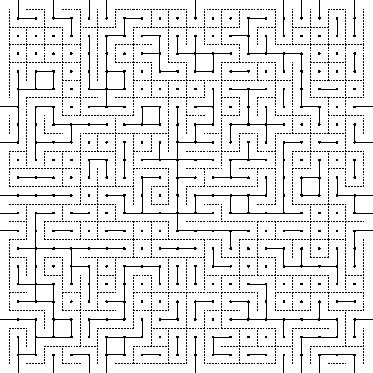
\includegraphics{torusrare}
    \caption{When $p = 0.33 < 1/3$, long cycles are rare. Dotted lines show
      missing edges in the dual.}
    \figlabel{peierlsrare}
  \end{subfigure}
  \quad\quad
  \begin{subfigure}[t]{0.4\textwidth}
    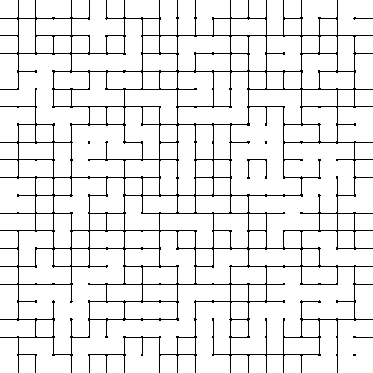
\includegraphics{torusdense}
    \caption{When $p = 0.67 > 2/3$, there is likely only one large
      component.}
  \end{subfigure}
  \caption{Random subgraphs of the $20 \times 20$ torus grid graph.}
  \figlabel{peierls}
\end{figure}

\subsection{Triangles in $G_{n,p}$}

Recall that the Erd\H{o}s-R\'{e}nyi random graph $G_{n,p}$ is the
space of graphs with vertex set $V=\{1,\ldots,n\}$ and in which each
edge $\{u, w\} \in \binom{V}{2}$ is present with probability $p$ and
absent with probability $1-p$, independently of the other edges.

The expected number of triangles (cycles of length 3) in $G_{n,p}$ is
easily seen to be $p^3\binom{n}{3}$.  For $p=(6c)^{1/3}/n$, this
expectation is $k-O(1/n)$.  Unfortunately, even when $c$ is a large
constant, it still takes some work to show that there is a constant
probability that $G_{n,p}$ contains at least one triangle. Indeed,
this typically requires the use of the second moment method, which
involves computing the variance of the number of triangles in
$G_{n,p}$. To show that $G_{n, p}$ has a triangle with exponential
probability is even more complicated, and a proof of this result would
still typically rely on an advanced probabilistic
inequality~\cite{alon:probabilistic}. Here we show how this can be
accomplished with an encoding argument.

\begin{thm}\thmlabel{triangles-up}
  For $p=c/n$, $G \in G_{n,p}$ contains at least one triangle with
  probability at least $1-2^{-\Omega(c^3)}$.
\end{thm}

\begin{proof}
  In this argument, we will produce an encoding of $G$'s adjacency
  matrix, $A$.

  Refer to \figref{triangles}.  If $G$ contains no triangles, then we
  look at the number of ones in the $n/2\times n/2$ submatrix $M$
  determined by rows $1,\ldots,n/2$ and columns $n/2+1,\ldots,n$. Note
  that $n_1(M)$, the number of ones in $M$, is a
  $\mathrm{Binomial}(n^2/4, c/n)$ random variable.  There are two
  cases to consider:
  
  \begin{figure}
    \centering{\includegraphics{triangles}}
    \caption{The random graph $G_{n,c/n}$ contains triangles when $c$
      is large enough.  The highlighted 0 bits in the last five rows
      can be deduced from pairs of 1 bits in the first 5 rows.}
    \figlabel{triangles} 
  \end{figure}

  \begin{enumerate}\setcounter{enumi}{-1}
  \item The number of ones in $M$ is less than $cn/8$.  In this case,
    the number of ones in this submatrix is much less than the
    expected number, $cn/4$.  Here one can apply the same argument
    used to prove Chernoff's bound (\thmref{chernoff}) or simply apply
    Chernoff's bound. We leave this as an exercise to the reader.

  \item The number of ones in the submatrix is greater than $cn/8$.
    Notice that, for $i<j<k$ if $A_{i,j}=1$ and $A_{i,k}=1$, then the
    fact that there are no triangles implies that $A_{j,k}=0$.

    Let $m_i$ be the number of ones in the $i$\textsuperscript{th} row
    of the submatrix.  By specifying rows $1,\ldots,n/2$, we eliminate
    the need to specify
    \[
      m = \sum_{i=1}^{n/2}\binom{m_i}{2} \ge (n/2) \binom{2
        n_1(M)/n}{2} \ge (n/2)\binom{c/4}{2} = \Omega(c^2n) \enspace ,
    \]
    zeros in rows $n/2+1,\ldots,n$. We thus encode $G$ by giving a
    Shannon-Fano code with parameter $p$ for the first $n/2$ rows of
    $A$; and a Shannon-Fano code with parameter $p$ for the rest of
    $A$, excluding the bits which can be deduced from the preceding
    information. Such a code has length
    \[
      |C(G)| = n_1(A) \log(1/p) + (n_0(A)-m)\log(1/(1-p))
    \]
    which results in a savings of
    \[
      s = \log(1/p_G) - |C(G)| = m\log(1/(1-p)) \ge
      \Omega(c^2n)\log(1/(1-p)) = \Omega(c^3) \enspace . \qedhere
    \]
  \end{enumerate}
\end{proof}

\begin{thm}\thmlabel{triangles-down}
  When $p = 1/(\alpha n)$, $G \in G_{n, p}$ has no triangle with
  probability at least $1 - \alpha^{-3}$.
\end{thm}
\begin{proof}
  Suppose that $G$ contains a triangle. We encode the adjacency matrix
  $A$ of $G$. First, we specify the triangle's vertices; and finish
  with a Shannon-Fano code with parameter $p$ for the remaining
  vertices of the graph. This code has length
  \begin{align*}
    |C(G)| &= 3 \log n + (n_1(A) - 3) \log (1/p) + n_0(A) \log (1/(1 - p)) \\
           &= \log (1/p_G) + 3 \log n - 3 \log (1/p) \\
           &= \log (1/p_G) - 3 \log \alpha \\
           &= \log (1/p_G) - \log \alpha^3 \enspace . \qedhere
  \end{align*}
\end{proof}

Together, \thmref{triangles-up} and \thmref{triangles-down} establish
that $1/n$ is a threshold function for triangle-freeness.

\section{Encoding with Kraft's Condition}
\seclabel{el}

We finally discuss why it has made sense to omit ceilings in all of
our encoding arguments.

Let $[0, \infty]$ denote the set of extended non-negative real
numbers, supporting all the usual extended arithmetic operations and
identities, including $1/0 = \infty$. Recall that a function
$\ell : X \to [0, \infty]$ \emph{satisfies Kraft's condition} if
\[
  \sum_{x \in X} 2^{-\ell(x)} \leq 1 \enspace .
\]

Observe that neither the (Non-)Uniform Encoding Lemma nor any of its
applications has required the specification of any prefix-free code:
We know, by construction, that every such code is prefix-free, but we
could also deduce from Kraft's inequality that, since our described
codes satisfy Kraft's condition, a prefix-free code with the same
codeword lengths exists. Instead, we will see that codeword lengths
satisfying Kraft's condition suffice, and such codeword lengths need
not be integers.

\begin{lem}\lemlabel{el}
  Let $\ell : X \to [0, \infty]$ satisfy Kraft's condition and let
  $x\in X$ be drawn randomly where $p_x$ denotes the probability of
  drawing $x$.  Then
  \[
    \Pr\{ \ell(x) \le \log(1/p_x)-s\} \le 2^{-s} \enspace .
  \]
\end{lem}
\begin{proof}
  The proof is identical to that of \lemref{nuel}.
\end{proof}

The sum of functions $\ell : X \to [0, \infty]$ and
$\ell' : X' \to [0, \infty]$ is the function
$\ell + \ell' : X \times X' \to [0, \infty]$, where
$(\ell + \ell') (x, x') = \ell(x) + \ell'(x')$. Note that for any
partial codes
$C : X \nrightarrow \{0, 1\}^*, C' : X' \nrightarrow \{0, 1\}^*$, any
$x \in X$, and any $x' \in X'$,
\[
(|C| + |C'|)(x, x') = |C(x)| + |C'(x')| = |(C \cdot C')|(x, x') \enspace .
\]
In other words, the sum of these functions describes the length of
codewords in composed codes.

\begin{lem}\lemlabel{composition-tight}
  If $\ell : X \to [0, \infty]$ and $\ell' : X' \to [0,
  \infty]$ satisfy Kraft's condition, then so does $\ell + \ell'$.
\end{lem}
\begin{proof}
  Kraft's condition still holds:
  \[
  \sum_{(x, x') \in X \times X'} 2^{-(\ell + \ell')(x, x')} = \sum_{x
    \in X} \sum_{x' \in X'} 2^{-\ell(x) - \ell'(x')} = \sum_{x \in X}
  2^{-\ell(x)} \sum_{x' \in X'} 2^{-\ell'(x')} \leq 1 \enspace
  . \qedhere
  \]
\end{proof}
This is analogous to the fact that the composition of prefix-free
codes is prefix-free.

\begin{lem}\lemlabel{fixed-length-tight}
  For any probability density $p : X \to [0, 1]$, the function
  $\ell : X \to [0, \infty]$ with $\ell(x) = \log (1/p_x)$
  satisfies Kraft's condition.
\end{lem}
\begin{proof}
  \[
  \sum_{x \in X} 2^{-\ell(x)} = \sum_{x \in X} 2^{-\log (1/p_x)} =
  \sum_{x \in X} p_x = 1 \enspace . \qedhere
  \]
\end{proof}
This tells us that we can ignore the ceiling in every instance of a
fixed-length code and every instance of a Shannon-Fano code while
encoding.

We now give a tight notion corresponding to Elias codes.
\begin{thm}[Beigel~\cite{beigel:elias}]\thmlabel{elias-tight}
  Fix some $0 < \eps < e - 1$. Let $\ell : \N \to \R$ have
  \[
  \ell(i) = \log i + \log \log i + \cdots + \underbrace{\log \cdots
    \log}_{\text{$\log^* i$ times}} i - (\log \log (e - \eps)) \log^*
  i + O(1) \enspace .
  \]
  Then, $\ell$ satisfies Kraft's condition. Moreover, the function
  $\ell' : \N \to \R$ with
  \[
  \ell'(i) = \log i + \log \log i + \cdots + \underbrace{\log \cdots
    \log}_{\text{$\log^* i$ times}} i - (\log \log e) \log^* i + c
  \]
  does not satisfy Kraft's condition for any choice of the constant
  $c$.
\end{thm}

It is not hard to see how \lemref{el}, \lemref{composition-tight},
\lemref{fixed-length-tight}, and \thmref{elias-tight} can be used to
give encoding arguments with real-valued codeword lengths. Indeed,
recall how the result of \thmref{runs-i} carried an artifact of binary
encoding. Using our new tools, we can now refine this and recover the
exact result.
\begin{customthm}{\ref*{thm:runs-i}b}
  Let $x=(x_1,\ldots,x_n)\in\{0,1\}^n$ be chosen uniformly at random
  and let $t = \ceil{\log n + s}$. Then, the probability that there
  exists an $i\in\{1,\ldots,n-t+1\}$ such that
  $x_i=x_{i+1}=\cdots=x_{i+t-1}=1$ is at most $2^{-s}$.
\end{customthm}
\begin{proof}
  Let $\ell : \{0, 1\}^n \to [0, \infty]$ be such that if $x$ contains
  a run of $t = \ceil{\log n + s}$ ones, then
  $\ell(x) = \log n + n - t$, and otherwise $\ell(x) = \infty$. We
  will show that $\ell$ satisfies Kraft's condition.

  %Recall that $x$ is said to contain a run of $t$ ones if there exists
  %some $i \in \{1, \ldots, n - t + 1\}$ such that $x_i = \cdots = x_{i
  %  + t - 1} = 1$.

  Let the function $f : \{1, \ldots, n - t + 1\} \to [0, \infty]$ have
  $f(i) = \log n$ for all $i$, and
  $g : \{0, 1\}^{n - t} \to [0, \infty]$ have $g(y) = n - t$ for all
  $y$. Both of these functions satisfy Kraft's condition by
  \lemref{fixed-length-tight}. By \lemref{composition-tight}, so does
  the function
  \[
    h = f + g : \{1, \ldots, n - t + 1\} \times \{0, 1\}^{n - t} \to
    [0, \infty] \enspace ,
  \]
  where $h(i, y) = \log n + n - t$ for all $i$ and $y$. Crucially,
  each element of the set $\{1, \ldots, n - t + 1\} \times \{0, 1\}^{n
    - t}$ corresponds to an $n$-bit binary string containing a run of
  $t$ ones: the element $(i, y) \in \{1, \ldots, n - t + 1\} \times
  \{0, 1\}^{n - t}$, where $y = (y_1, \ldots, y_{n - t})$, corresponds
  to the binary string
  \[
  (y_1, \dots, y_{i - 1}, \underbrace{1, 1, \dots, 1}_{\text{$t$ times}},
  y_i, \dots, y_{n - t}) \enspace .
  \]
  Therefore, $\ell$ satisfies Kraft's condition. By our choice of
  $t$, we have that $\ell(x) \leq n - s$ if and only if $x$ contains a
  run of $t$ ones. We finish by applying \lemref{el}.
\end{proof}

\section{Summary and Conclusions}
\seclabel{summary}

We have described a simple method for producing encoding
arguments. Using our encoding lemmas, we gave original proofs for
several previously established results.

Typically, one would invoke the incompressibility method after
developing some of the theory of Kolmogorov complexity. Our technique
requires only a basic understanding of prefix-free codes and one
simple lemma. We are also the first to suggest a simple and tight
manner of encoding using only Kraft's condition with real-valued
codeword lengths. In this light, we posit that there is no reason to
develop an encoding argument through the incompressibility method: our
Uniform Encoding Lemma is simpler, the Non-Uniform Encoding Lemma is
more general, and our technique from \secref{el} is less
wasteful. Indeed, though it would be easy to state and prove our
Non-Uniform Encoding Lemma in the setting of Kolmogorov complexity, it
seems as if the general encoding lemma from \secref{el} only can exist
in our simplified framework.

\begin{comment}
Using our encoding lemmas, we gave original proofs for several
previously established results. Specifically, we showed:
\begin{itemize}
\item if $n$ balls are thrown into $n$ urns uniformly at random, then
  no urn contains more than $O(\log n/\log \log n)$ balls with high
  probability;
\item linear probing succeeds in $O(1)$ expected time;
\item searching in 2-choice hashing takes time $O(\log \log n)$ with
  high probability;
\item a certain random bipartite graph is an expander with high
  probability;
\item the number of records in a uniformly random permutation is
  $O(\log n)$ with high probability;
\item the height of the binary search tree built from the sequential
  insertion of a uniformly random permutation of $n$ integers is
  $O(\log n)$ with high probability;
\item Chernoff's bound on the tail of a binomial random variable;
\item percolation occurs in random dense subgraphs of the torus;
\item a strong threshold for triangle-freeness in the
  Erd\H{o}s-R\'{e}nyi random graph.
\end{itemize}
\end{comment}

\section*{Acknowledgement}

This research was initiated in response to an invitation for the first
author to give a talk at the Ninth Annual Probability, Combinatorics
and Geometry Workshop, held April 4--11 at McGill University's
Bellairs Institute.  Many ideas that appear in the current paper were
developed during the workshop. The author is grateful to the other
workshop participants for providing a stimulating working environment.
In particular, Xing~Shi~Cai pointed out the application to runs in
binary strings (\thmref{runs-i}) and G\'abor~Lugosi stated and proved
the Non-Uniform Encoding Lemma (\lemref{nuel}) in response to the first
author's half-formed ideas about a non-uniform version of \lemref{uel}.

\bibliography{encoding}{}
\bibliographystyle{plain}

\end{document}
